\chapter{Uncertainty Quantification Capabilities}\label{uq}

\section{Overview}\label{uq:overview}

Uncertainty quantification (UQ) is the process of determining the
effect of input uncertainties on response metrics of interest.  These
input uncertainties may be characterized as either aleatory
uncertainties, which are irreducible variabilities inherent in nature,
or epistemic uncertainties, which are reducible uncertainties
resulting from a lack of knowledge.  Since sufficient data is
generally available for aleatory uncertainties, probabilistic methods
are commonly used for computing response distribution statistics based
on input probability distribution specifications.  Conversely, for
epistemic uncertainties, data is generally sparse, making the use of
probability distribution assertions questionable and typically leading
to nonprobabilistic methods based on interval specifications.

DAKOTA contains capabilities for performing nondeterministic analysis.
The methods for uncertainty quantification in DAKOTA have been
developed by a group of researchers at Sandia Labs, in conjunction
with collaborators in academia~\cite{Gha99,Gha91,Eld05,Tang10a}.
%In addition, future extensions to the DDACE package will make it 
%applicable to general UQ problems, which will augment the DAKOTA/UQ 
%capabilities.
%Uncertainty quantification methods (also referred to as
%nondeterministic analysis methods) in the DAKOTA/UQ system involve the
%computation of probabilistic information about response functions
%based on sets of simulations taken from the specified probability
%distributions for uncertain parameters. That is, 
These methods perform a forward uncertainty propagation in which
probability or interval information for input parameters is mapped to
probability or interval information for output response functions. The
$m$ functions in the DAKOTA response data set are interpreted as $m$
general response functions by the DAKOTA methods (with no specific
interpretation of the functions as for optimization and least squares).

Within the variables specification, uncertain variable descriptions
are employed to define the parameter probability distributions (see
Section~\ref{variables:uncertain}). The continuous aleatory
distribution types include: normal (Gaussian), lognormal, uniform,
loguniform, triangular, exponential, beta, gamma, gumbel, frechet,
weibull, and histogram bin.  The discrete aleatory distribution types
include: poisson, binomial, negative binomial, geometric,
hypergeometric, and histogram point.  The epistemic distribution type
is interval.  When gradient and/or Hessian information is used in an
uncertainty assessment, derivative components are normally computed
with respect to the active continuous variables, or in this case, the
\emph{continuous uncertain variables} (aleatory, epistemic, 
or both, excluding \texttt{all\_variables} mode; see 
Section~\ref{responses:active}).

\section{Sampling Methods}\label{uq:sampling}

Sampling techniques are selected using the \texttt{sampling}
method selection. This method generates sets of samples according to
the probability distributions of the uncertain variables and maps them
into corresponding sets of response functions, where the number of
samples is specified by the \texttt{samples} integer specification.
Means, standard deviations, coefficients of variation (COVs), and 95\%
confidence intervals are computed for the response functions.
Probabilities and reliabilities may be computed for 
\texttt{response\_levels} specifications, and response levels may be
computed for either \texttt{probability\_levels} or
\texttt{reliability\_levels} specifications (refer to the Method
Commands chapter in the DAKOTA Reference Manual~\cite{RefMan} for
additional information).

Currently, traditional Monte Carlo (MC) and Latin hypercube sampling
(LHS) are supported by DAKOTA and are chosen by specifying
\texttt{sample\_type} as \texttt{random} or \texttt{lhs}. In Monte
Carlo sampling, the samples are selected randomly according to the
user-specified probability distributions. Latin hypercube sampling is
a stratified sampling technique for which the range of each uncertain
variable is divided into $N_{s}$ segments of equal probability, where
$N_{s}$ is the number of samples requested. The relative lengths of
the segments are determined by the nature of the specified probability
distribution (e.g., uniform has segments of equal width, normal has
small segments near the mean and larger segments in the tails). For
each of the uncertain variables, a sample is selected randomly from
each of these equal probability segments.  These $N_{s}$ values for
each of the individual parameters are then combined in a shuffling
operation to create a set of $N_{s}$ parameter vectors with a
specified correlation structure. A feature of the resulting sample set
is that 
\emph{every row and column in the hypercube of partitions has exactly one sample}.
Since the total number of samples is exactly equal
to the number of partitions used for each uncertain variable, an
arbitrary number of desired samples is easily accommodated (as
compared to less flexible approaches in which the total number of
samples is a product or exponential function of the number of
intervals for each variable, i.e., many classical design of
experiments methods).

Advantages of sampling-based methods include their relatively simple
implementation and their independence from the scientific disciplines
involved in the analysis. The main drawback of these techniques is the
large number of function evaluations needed to generate converged
statistics, which can render such an analysis computationally very
expensive, if not intractable, for real-world engineering
applications. LHS techniques, in general, require fewer samples than
traditional Monte Carlo for the same accuracy in statistics, but they
still can be prohibitively expensive. For further information on the
method and its relationship to other sampling techniques, one is
referred to the works by McKay, et al.~\cite{Mck79}, Iman and
Shortencarier~\cite{Ima84}, and Helton and Davis~\cite{Hel00}.
Note that under certain separability conditions associated with the 
function to be sampled,
Latin hypercube sampling provides a more accurate estimate of the mean
value than does random sampling. That is, given an equal number of
samples, the LHS estimate of the mean will have less variance than the
mean value obtained through random sampling.

Figure~\ref{dace:figure01} demonstrates Latin hypercube sampling on a
two-variable parameter space. Here, the range of both parameters,
$x_1$ and $x_2$, is $[0,1]$. Also, for this example both $x_1$
and $x_2$ have uniform statistical distributions.  For Latin
hypercube sampling, the range of each parameter is divided into $p$
``bins'' of equal probability. For parameters with uniform
distributions, this corresponds to partitions of equal size. For $n$
design parameters, this partitioning yields a total of $p^{n}$ bins in
the parameter space.  Next, $p$ samples are randomly selected in the
parameter space, with the following restrictions: (a) each sample is
randomly placed inside a bin, and (b) for all one-dimensional
projections of the $p$ samples and bins, there will be one and only
one sample in each bin.  In a two-dimensional example such as that
shown in Figure~\ref{dace:figure01}, these LHS rules guarantee that
only one bin can be selected in each row and column. For $p=4$, there
are four partitions in both $x_1$ and $x_2$. This gives a total of
16 bins, of which four will be chosen according to the criteria
described above. Note that there is more than one possible arrangement
of bins that meet the LHS criteria.  The dots in
Figure~\ref{dace:figure01} represent the four sample sites in this
example, where each sample is randomly located in its bin.  There is
no restriction on the number of bins in the range of each parameter,
however, all parameters must have the same number of bins.

\begin{figure}
  \centering
  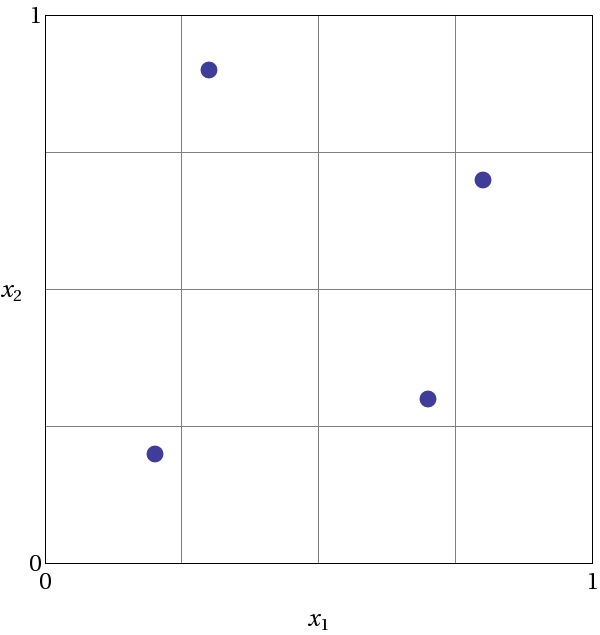
\includegraphics[scale=0.35]{images/lhs_graphic}
  \caption{An example of Latin hypercube sampling with four bins in
    design parameters $x_1$ and $x_2$. The dots
    are the sample sites.}
  \label{dace:figure01}
\end{figure}

The actual algorithm for generating Latin hypercube samples is more
complex than indicated by the description given above. For example,
the Latin hypercube sampling method implemented in the LHS
code~\cite{Swi04} takes into account a user-specified correlation
structure when selecting the sample sites. For more details on the
implementation of the LHS algorithm, see Reference~\cite{Swi04}.

\subsection{Uncertainty Quantification Example using Sampling Methods}\label{uq:uncertainty1}

The two-variable Textbook example problem (see
Equation~\ref{tutorial:textbook_f}) will be used to demonstrate
the application of sampling methods for uncertainty quantification
where it is assumed that $x_1$ and $x_2$ are uniform uncertain
variables on the interval $[0,1]$. The DAKOTA input file for this
problem is shown in Figure~\ref{uq:figure01}. This input 
file is \texttt{dakota\_uq\_sampling.in} in the 
\texttt{Dakota/examples/methods} directory.  The number of samples to
perform is controlled with the \texttt{samples} specification, the
type of sampling algorithm to use is controlled with the
\texttt{sample\_type} specification, the levels used for computing
statistics on the response functions is specified with the
\texttt{response\_levels} input, and the \texttt{seed} specification
controls the sequence of the pseudo-random numbers generated by the
sampling algorithms. The input samples generated are shown in
Figure~\ref{uq:figure02} for the case where \texttt{samples} = 5 and
\texttt{samples} = 10 for both \texttt{random} ($\circ$) and 
\texttt{lhs} ($+$) sample types.

\begin{figure}
  \centering \begin{bigbox} \begin{small}
  \verbatimtabinput[8]{dakota_uq_sampling.in} \end{small} \end{bigbox}
\caption{DAKOTA input file for UQ example using LHS sampling.}
\label{uq:figure01}
\end{figure}

\begin{figure}
  \centering
  \subfigure{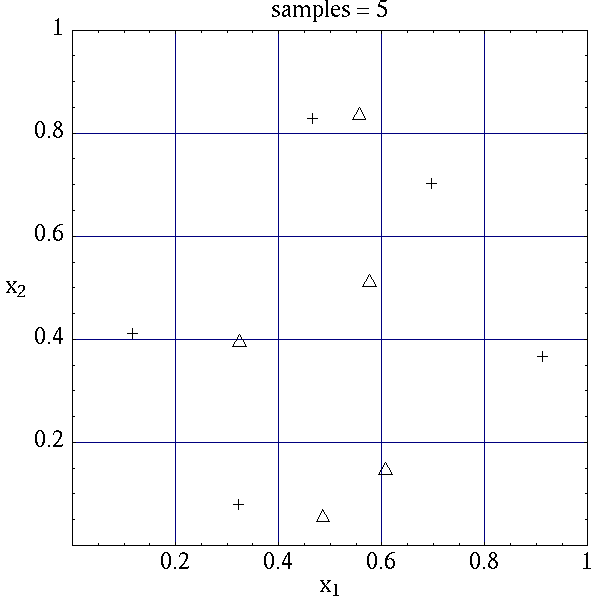
\includegraphics[scale=0.35]{images/input_samples5}}
  \subfigure{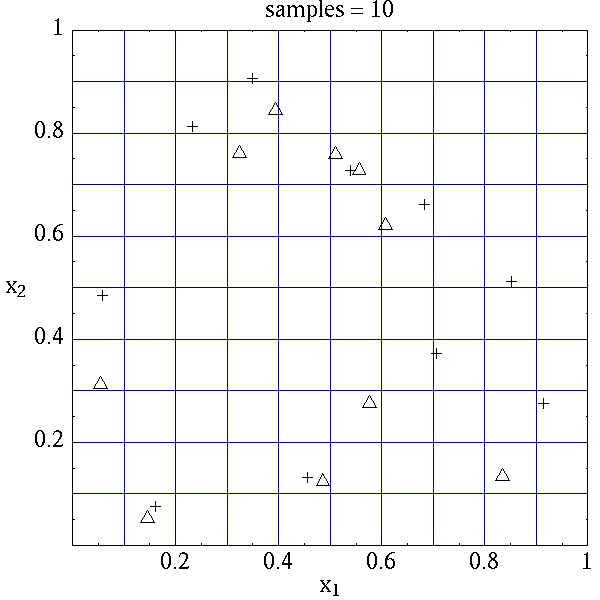
\includegraphics[scale=0.35]{images/input_samples10}}
  \caption{Distribution of input sample points for random ($\triangle$)
    and lhs ($+$) sampling for \texttt{samples=5} and \texttt{10}.}
  \label{uq:figure02}
\end{figure}

Latin hypercube sampling ensures full coverage of the range of the
input variables, which is often a problem with Monte Carlo sampling
when the number of samples is small. In the case of \texttt{samples =
5}, poor stratification is evident in $x_1$ as four out of the five
Monte Carlo samples are clustered in the range $0.35 < x_1 < 0.55$,
and the regions $x_1 < 0.3$ and $0.6 < x_1 < 0.9$ are completely
missed. For the case where \texttt{samples = 10}, some clustering in
the Monte Carlo samples is again evident with \texttt{4} samples in
the range $0.5 < x_1 < 0.55$. In both cases, the stratification with
LHS is superior.  The response function statistics returned by DAKOTA
are shown in Figure~\ref{uq:figure03}.  The first two blocks of output
specify the response sample means and sample standard deviations and
confidence intervals for these statistics, as well as coefficients of
variation.  The last section of the output defines CDF pairs
(\texttt{distribution cumulative} was specified) for the response
functions by presenting the probability levels corresponding to the
specified response levels (\texttt{response\_levels} were set and the
default \texttt{compute probabilities} was used).  Alternatively,
DAKOTA could have provided CCDF pairings, reliability levels
corresponding to prescribed response levels, or response levels
corresponding to prescribed probability or reliability levels.

\begin{figure}
\centering
\begin{bigbox}
\begin{small}
\begin{verbatim}
Statistics based on 10 samples:

Moments for each response function:
response_fn_1:  Mean = 3.83840e-01  Std. Dev. = 4.02815e-01
                Coeff. of Variation = 1.04944e+00
response_fn_2:  Mean = 7.47987e-02  Std. Dev. = 3.46861e-01
                Coeff. of Variation = 4.63726e+00
response_fn_3:  Mean = 7.09462e-02  Std. Dev. = 3.41532e-01
                Coeff. of Variation = 4.81397e+00

95% confidence intervals for each response function:
response_fn_1:  Mean = (  9.56831e-02, 6.71997e-01 ),
             Std Dev = (  2.77071e-01, 7.35384e-01 )
response_fn_2:  Mean = ( -1.73331e-01, 3.22928e-01 ),
             Std Dev = (  2.38583e-01, 6.33233e-01 )
response_fn_3:  Mean = ( -1.73371e-01, 3.15264e-01 ),
             Std Dev = (  2.34918e-01, 6.23505e-01 )

Probabilities for each response function:
Cumulative Distribution Function (CDF) for response_fn_1:
     Response Level  Probability Level  Reliability Index
     --------------  -----------------  -----------------
   1.0000000000e-01   3.0000000000e-01
   2.0000000000e-01   5.0000000000e-01
   6.0000000000e-01   7.0000000000e-01
Cumulative Distribution Function (CDF) for response_fn_2:
     Response Level  Probability Level  Reliability Index
     --------------  -----------------  -----------------
   1.0000000000e-01   5.0000000000e-01
   2.0000000000e-01   7.0000000000e-01
   6.0000000000e-01   9.0000000000e-01
Cumulative Distribution Function (CDF) for response_fn_3:
     Response Level  Probability Level  Reliability Index
     --------------  -----------------  -----------------
   1.0000000000e-01   6.0000000000e-01
   2.0000000000e-01   6.0000000000e-01
   6.0000000000e-01   9.0000000000e-01
\end{verbatim}
\end{small}
\end{bigbox}
\caption{DAKOTA response function statistics from UQ sampling example.}
\label{uq:figure03}
\end{figure}

In addition to obtaining statistical summary information of the type
shown in Figure~\ref{uq:figure03}, the results of LHS sampling also
include correlations.  Four types of correlations are returned in the
output: simple and partial ``raw'' correlations, and simple and
partial ``rank'' correlations.  The raw correlations refer to
correlations performed on the actual input and output data.  Rank
correlations refer to correlations performed on the ranks of the data.
Ranks are obtained by replacing the actual data by the ranked values,
which are obtained by ordering the data in ascending order.  For
example, the smallest value in a set of input samples would be given a
rank 1, the next smallest value a rank 2, etc.  Rank correlations are
useful when some of the inputs and outputs differ greatly in
magnitude: then it is easier to compare if the smallest ranked input
sample is correlated with the smallest ranked output, for example.

Correlations are always calculated between two sets of sample data.
One can calculate correlation coefficients between two input
variables, between an input and an output variable (probably the most
useful), or between two output variables.  The simple correlation
coefficients presented in the output tables are Pearson's correlation
coefficient, which is defined for two variables $x$ and $y$ as:
$\mathtt{Corr}(x,y) = \frac{\sum_{i}(x_{i}-\bar{x})(y_{i}-\bar{y})}
{\sqrt{\sum_{i}(x_{i}-\bar{x})^2\sum_{i}(y_{i}-\bar{y})^2}}$.
Partial correlation coefficients are similar to simple correlations,
but a partial correlation coefficient between two variables measures
their correlation while adjusting for the effects of the other
variables.  For example, say one has a problem with two inputs and one
output; and the two inputs are highly correlated.  Then the
correlation of the second input and the output may be very low after
accounting for the effect of the first input.  The rank correlations
in DAKOTA are obtained using Spearman's rank correlation.  Spearman's
rank is the same as the Pearson correlation coefficient except that it
is calculated on the rank data.

Figure~\ref{uq:figure04} shows an example of the correlation output
provided by DAKOTA for the input file in Figure~\ref{uq:figure01}.
Note that these correlations are presently only available when one
specifies \texttt{lhs} as the sampling method under \texttt{sampling}.
Also note that the simple and partial correlations should be similar in most
cases (in terms of values of correlation coefficients).  This is
because we use a default ``restricted pairing'' method in the LHS
routine which forces near-zero correlation amongst uncorrelated
inputs.

\begin{figure}
\centering
\begin{bigbox}
\begin{small}
\begin{verbatim}
Simple Correlation Matrix between input and output:
                       x1           x2 response_fn_1 response_fn_2 response_fn_3
          x1  1.00000e+00
          x2 -7.22482e-02  1.00000e+00
response_fn_1 -7.04965e-01 -6.27351e-01  1.00000e+00
response_fn_2  8.61628e-01 -5.31298e-01 -2.60486e-01  1.00000e+00
response_fn_3 -5.83075e-01  8.33989e-01 -1.23374e-01 -8.92771e-01  1.00000e+00

Partial Correlation Matrix between input and output:
             response_fn_1 response_fn_2 response_fn_3
          x1 -9.65994e-01  9.74285e-01 -9.49997e-01
          x2 -9.58854e-01 -9.26578e-01  9.77252e-01

Simple Rank Correlation Matrix between input and output:
                       x1           x2 response_fn_1 response_fn_2 response_fn_3
          x1  1.00000e+00
          x2 -6.66667e-02  1.00000e+00
response_fn_1 -6.60606e-01 -5.27273e-01  1.00000e+00
response_fn_2  8.18182e-01 -6.00000e-01 -2.36364e-01  1.00000e+00
response_fn_3 -6.24242e-01  7.93939e-01 -5.45455e-02 -9.27273e-01  1.00000e+00

Partial Rank Correlation Matrix between input and output:
             response_fn_1 response_fn_2 response_fn_3
          x1 -8.20657e-01  9.74896e-01 -9.41760e-01
          x2 -7.62704e-01 -9.50799e-01  9.65145e-01
\end{verbatim}
\end{small}
\end{bigbox}
\caption{Correlation results using LHS Sampling.}
\label{uq:figure04}
\end{figure}

Finally, note that the LHS package can be used for design of
experiments over design and state variables by including the
\texttt{all\_variables} flag in the method specification section of
the DAKOTA input file. Then, instead of iterating on only the
uncertain variables, the LHS package will sample over all of the
variables.  In \texttt{all\_variables} mode, continuous design and
continuous state variables are treated as having uniform probability
distributions within their upper and lower bounds, discrete values are
sampled uniformly from within their sets or ranges, and any uncertain
variables are sampled within their specified probability distributions.

\subsection{Incremental Sampling}\label{uq:incremental}

In many situations, one may run an initial sample set and then need to
perform further sampling to get better estimates of the mean,
variance, and percentiles, and to obtain more comprehensive sample
coverage.  We call this capability incremental sampling. Currently,
the LHS incremental sampling capability we have in DAKOTA requires that
the incremental samples are double the sample size of the previous
sample.  That is, if one starts with a very small sample size of 10,
then one can use the incremental sampling capability to generate
sample sizes of 20, 40, 80, etc. Also, a DAKOTA restart file
(dakota.rst) must be available from the original sample. There are two
cases, random incremental and Latin Hypercube incremental sampling.
We assume that LHS incremental will be most frequently used.  One
major advantage of LHS incremental sampling is that it maintains the
stratification and correlation structure of the original LHS sample.
That is, if one generated 2 independent LHS samples and just merged
them, the calculation of the accuracy of statistical measures such as
the mean and the variance would be slightly incorrect.  However, in
the incremental case, the full sample (double the original size) is a
Latin Hypercube sample itself and statistical measures and their
accuracy can be properly calculated.  The incremental sampling
capability is most useful when one is starting off with very small
samples. Once the sample size is more than a few hundred, the benefit
of incremental sampling diminishes.

\begin{enumerate}

\item Incremental Random Sampling.  With incremental random sampling, 
the original sample set with N samples must be 
generated using \texttt{sample\_type} as \texttt{random}.
Then, the user can create a new DAKOTA input file that is very similar to the 
original one except the \texttt{sample\_type} should be defined to be 
\texttt{incremental\_random}.  Random incremental sampling does not 
require a doubling of samples each time.  Thus, the user 
can specify the number of samples (\texttt{samples}) to be a desired 
number (it can range from an additional one sample to a large integer), 
and the \texttt{previous\_samples} should be specified as N.  For example, if
the first sample has 50 samples, and 10 more samples are desired, 
in the second DAKOTA run, the number
of samples should be set to 60 and the number of previous samples set
to 50.  In this situation, only 10 new samples will be generated and
the final statistics will be reported on the full sample of 60. The
command line syntax for running the second sample is \texttt{dakota -i
input2.in -r dakota.rst} where input2.in is the input file with the
incremental sampling specification and dakota.rst is the restart file.
Note that if the restart file has a different name, that is fine; the
correct restart file name should be used.

\item Incremental Latin Hypercube Sampling. With incremental LHS sampling, 
the original sample set with N samples must be 
generated using \texttt{sample\_type} as \texttt{lhs}.
Then, the user can create a new DAKOTA input file that is very similar to the 
original one except the \texttt{sample\_type} should be defined to be 
\texttt{incremental\_lhs}, the number of samples (\texttt{samples}) should 
be 2N (twice the number of original samples), and
\texttt{previous\_samples} should be specified as N.  For example, if
the first sample has 50 samples, in the second DAKOTA run, the number
of samples should be set to 100 and the number of previous samples set
to 50.  In this situation, only 50 new samples will be generated and
the final statistics will be reported on the full sample of 100. The
command line syntax for running the second sample is \texttt{dakota -i
input2.in -r dakota.rst}, where input2.in is the input file with the
incremental sampling specification and dakota.rst is the restart file.
Note that if the restart file has a different name, that is fine; the
correct restart file name should be used.

\end{enumerate}

\section{Reliability Methods}\label{uq:reliability}

Reliability methods provide an alternative approach to uncertainty
quantification which can be less computationally demanding than
sampling techniques.  Reliability methods for uncertainty
quantification are based on probabilistic approaches that compute
approximate response function distribution statistics based on
specified uncertain variable distributions.  These response statistics
include response mean, response standard deviation, and cumulative or
complementary cumulative distribution functions (CDF/CCDF).  These
methods are often more efficient at computing statistics in the tails
of the response distributions (events with low probability) than
sampling based approaches since the number of samples required to
resolve a low probability can be prohibitive.

The methods all answer the fundamental question: ``Given a set of
uncertain input variables, $\mathbf{X}$, and a scalar response
function, $g$, what is the probability that the response function is
below or above a certain level, $\bar{z}$?'' The former can be written
as $P[g(\mathbf{X}) \le \bar{z}] = \mathit{F}_{g}(\bar{z})$ where
$\mathit{F}_{g}(\bar{z})$ is the cumulative distribution function
(CDF) of the uncertain response $g(\mathbf{X})$ over a set of response
levels.  The latter can be written as $P[g(\mathbf{X}) > \bar{z}]$ and
defines the complementary cumulative distribution function (CCDF).

This probability calculation involves a multi-dimensional integral
over an irregularly shaped domain of interest, $\mathbf{D}$, where
$g(\mathbf{X}) < z$ as displayed in Figure~\ref{uq:figure05} for the
case of two variables.  The reliability methods all involve the
transformation of the user-specified uncertain variables,
$\mathbf{X}$, with probability density function, $p(x_1,x_2)$, which
can be non-normal and correlated, to a space of independent Gaussian
random variables, $\mathbf{u}$, possessing a mean value of zero and
unit variance (i.e., standard normal variables). The region of
interest, $\mathbf{D}$, is also mapped to the transformed space to
yield, $\mathbf{D_{u}}$ , where $g(\mathbf{U}) < z$ as shown in
Figure~\ref{uq:figure06}.  The Nataf transformation~\cite{Der86},
which is identical to the Rosenblatt transformation~\cite{Ros52} in
the case of independent random variables, is used in DAKOTA to
accomplish this mapping. This transformation is performed to make the
probability calculation more tractable. In the transformed space,
probability contours are circular in nature as shown in
Figure~\ref{uq:figure06} unlike in the original uncertain variable
space, Figure~\ref{uq:figure05}. Also, the multi-dimensional integrals
can be approximated by simple functions of a single parameter,
$\beta$, called the reliability index.  $\beta$ is the minimum
Euclidean distance from the origin in the transformed space to the
response surface. This point is also known as the most probable point
(MPP) of failure. Note, however, the methodology is equally applicable
for generic functions, not simply those corresponding to failure
criteria; this nomenclature is due to the origin of these methods
within the disciplines of structural safety and reliability.
Note that there are local and global reliability methods.  The majority 
of the methods available are local, meaning that a local optimization 
formulation is used to locate one MPP.  In contrast, global methods
can find multiple MPPs if they exist.
\begin{figure}
  \centering
  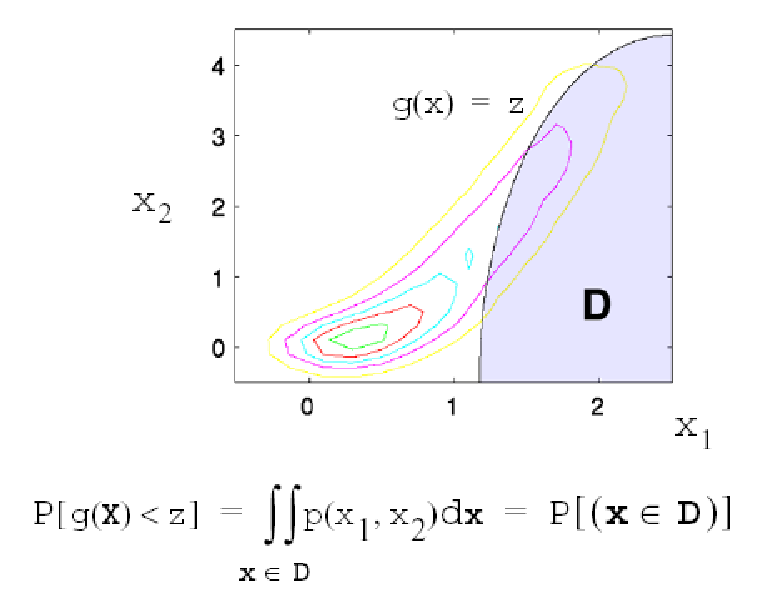
\includegraphics[scale=0.75]{images/cdf_orig_graphic}
  \caption{Graphical depiction of calculation of cumulative
    distribution function in the original uncertain variable space.}
  \label{uq:figure05}
\end{figure}

\begin{figure}
  \centering
  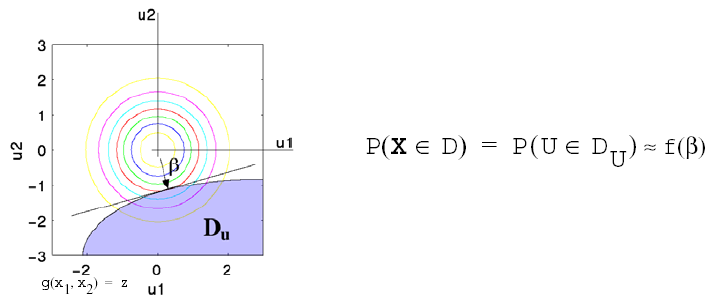
\includegraphics[scale=0.75]{images/cdf_tran_graphic}
  \caption{Graphical depiction of integration for the calculation of
    cumulative distribution function in the transformed uncertain
    variable space.}
  \label{uq:figure06}
\end{figure}

\subsection{Mean Value}\label{uq:reliability:mv}

The Mean Value method (MV, also known as MVFOSM in \cite{Hal00}) is
the simplest, least-expensive reliability method because it estimates
the response means, response standard deviations, and all CDF/CCDF
response-probability-reliability levels from a single evaluation of
response functions and their gradients at the uncertain variable
means.  This approximation can have acceptable accuracy when the
response functions are nearly linear and their distributions are
approximately Gaussian, but can have poor accuracy in other
situations.  The expressions for approximate response mean $\mu_g$,
approximate response variance $\sigma^2_g$, response target to
approximate probability/reliability level mapping ($\bar{z} \to p,\beta$),
and probability/reliability target to approximate response level mapping
($\bar{p},\bar{\beta} \to z$) are

\begin{eqnarray}
\mu_g      & = & g(\mu_{\bf x})  \label{eq:mv_mean1} \\
\sigma^2_g & = & \sum_i \sum_j Cov(i,j) \frac{dg}{dx_i}(\mu_{\bf x})
                 \frac{dg}{dx_j}(\mu_{\bf x}) \label{eq:mv_std_dev} \\
\beta_{cdf}  & = & \frac{\mu_g - \bar{z}}{\sigma_g} \label{eq:mv_ria_cdf} \\
\beta_{ccdf} & = & \frac{\bar{z} - \mu_g}{\sigma_g} \label{eq:mv_ria_ccdf} \\
z        & = & \mu_g - \sigma_g \bar{\beta}_{cdf} \label{eq:mv_pma_cdf} \\
z        & = & \mu_g + \sigma_g \bar{\beta}_{ccdf} \label{eq:mv_pma_ccdf}
\end{eqnarray}

respectively, where ${\bf x}$ are the uncertain values in the 
space of the original uncertain variables (``x-space''), $g({\bf x})$
is the limit state function (the response function for which
probability-response level pairs are needed), and $\beta_{cdf}$ and
$\beta_{ccdf}$ are the CDF and CCDF reliability indices, respectively.

With the introduction of second-order limit state information, MVSOSM
calculates a second-order mean as

\begin{equation}
\mu_g = g(\mu_{\bf x}) + \frac{1}{2} \sum_i \sum_j Cov(i,j) 
\frac{d^2g}{dx_i dx_j}(\mu_{\bf x}) \label{eq:mv_mean2}
\end{equation}

This is commonly combined with a first-order variance
(Equation~\ref{eq:mv_std_dev}), since second-order variance involves
higher order distribution moments (skewness, kurtosis)~\cite{Hal00}
which are often unavailable.

The first-order CDF probability $p(g \le z)$, first-order 
CCDF probability $p(g > z)$, $\beta_{cdf}$, and $\beta_{ccdf}$ are
related to one another through

\begin{eqnarray}
p(g \le z)   & = & \Phi(-\beta_{cdf})     \label{eq:p_cdf} \\
p(g > z)     & = & \Phi(-\beta_{ccdf})    \label{eq:p_ccdf} \\
\beta_{cdf}  & = & -\Phi^{-1}(p(g \le z)) \label{eq:beta_cdf} \\
\beta_{ccdf} & = & -\Phi^{-1}(p(g > z))   \label{eq:beta_ccdf} \\
\beta_{cdf}  & = & -\beta_{ccdf}          \label{eq:beta_cdf_ccdf} \\
p(g \le z)   & = & 1 - p(g > z)           \label{eq:p_cdf_ccdf}
\end{eqnarray}

where $\Phi()$ is the standard normal cumulative distribution
function.  A common convention in the literature is to define $g$ in
such a way that the CDF probability for a response level $z$ of zero
(i.e., $p(g \le 0)$) is the response metric of interest.  DAKOTA is
not restricted to this convention and is designed to support CDF or
CCDF mappings for general response, probability, and reliability level
sequences.

With the Mean Value method, it is possible to obtain 
importance factors indicating the relative importance of 
input variables.  The importance factors can be viewed
as an extension of linear sensitivity analysis combining deterministic
gradient information with input uncertainty information,
\emph{i.e}. input variable standard deviations. The accuracy of the
importance factors is contingent of the validity of the linear
approximation used to approximate the true response functions.
The importance factors are determined as: 

\begin{equation}
ImpFactor_i  = ({\frac{\sigma_{x_{i}}}{\sigma_g}}{\frac{dg}{dx_i}(\mu_{\bf x})})^2
\end{equation}


\subsection{MPP Search Methods}\label{uq:reliability:mpp}

All other local reliability methods solve an equality-constrained nonlinear
optimization problem to compute a most probable point (MPP) and then
integrate about this point to compute probabilities.  The MPP search
is performed in uncorrelated standard normal space (``u-space'') since
it simplifies the probability integration: the distance of the MPP
from the origin has the meaning of the number of input standard
deviations separating the mean response from a particular response
threshold.  The transformation from correlated non-normal
distributions (x-space) to uncorrelated standard normal distributions
(u-space) is denoted as ${\bf u} = T({\bf x})$ with the reverse
transformation denoted as ${\bf x} = T^{-1}({\bf u})$.  These
transformations are nonlinear in general, and possible approaches
include the Rosenblatt~\cite{Ros52}, Nataf~\cite{Der86}, and
Box-Cox~\cite{Box64} transformations.  The nonlinear transformations
may also be linearized, and common approaches for this include the
Rackwitz-Fiessler~\cite{Rac78} two-parameter equivalent normal and the
Chen-Lind~\cite{Che83} and Wu-Wirsching~\cite{Wu87} three-parameter
equivalent normals.  DAKOTA employs the Nataf nonlinear transformation
which is suitable for the common case when marginal distributions and
a correlation matrix are provided, but full joint distributions are
not known\footnote{If joint distributions are known, then the
Rosenblatt transformation is preferred.}.  This transformation occurs 
in the following two steps.  To transform between the
original correlated x-space variables and correlated standard normals
(``z-space''), a CDF matching condition is applied for each of the
marginal distributions:
\begin{equation}
\Phi(z_i) = F(x_i) \label{eq:trans_zx}
\end{equation}
where $F()$ is the cumulative distribution function of the original
probability distribution.  Then, to transform between correlated
z-space variables and uncorrelated u-space variables, the Cholesky 
factor ${\bf L}$ of a modified correlation matrix is used:
\begin{equation}
{\bf z} = {\bf L} {\bf u} \label{eq:trans_zu}
\end{equation}
where the original correlation matrix for non-normals in x-space has
been modified to represent the corresponding ``warped'' correlation in 
z-space~\cite{Der86}.

The forward reliability analysis algorithm of computing CDF/CCDF
probability/reliability levels for specified response levels is called
the reliability index approach (RIA), and the inverse reliability
analysis algorithm of computing response levels for specified CDF/CCDF
probability/reliability levels is called the performance measure
approach (PMA)~\cite{Tu99}.  The differences between the RIA and PMA
formulations appear in the objective function and equality constraint
formulations used in the MPP searches.  For RIA, the MPP search for
achieving the specified response level $\bar{z}$ is formulated as
computing the minimum distance in u-space from the origin to the
$\bar{z}$ contour of the limit state response function:
\begin{eqnarray}
{\rm minimize}     & {\bf u}^T {\bf u} \nonumber \\
{\rm subject \ to} & G({\bf u}) = \bar{z} \label{eq:ria_opt}
\end{eqnarray}

and for PMA, the MPP search for achieving the specified
reliability/probability level $\bar{\beta},\bar{p}$ is formulated as
computing the minimum/maximum response function value corresponding
to a prescribed distance from the origin in u-space:
\begin{eqnarray}
{\rm minimize}     & \pm G({\bf u}) \nonumber \\
{\rm subject \ to} & {\bf u}^T {\bf u} = \bar{\beta}^2 \label{eq:pma_opt}
\end{eqnarray}

where ${\bf u}$ is a vector centered at the origin in 
u-space and $g({\bf x}) \equiv G({\bf u})$ by definition.  In the RIA
case, the optimal MPP solution ${\bf u}^*$ defines the reliability 
index from $\beta = \pm \|{\bf u}^*\|_2$, which in turn defines the 
CDF/CCDF probabilities (using Equations~\ref{eq:p_cdf}-\ref{eq:p_ccdf} in 
the case of first-order integration).  The sign of $\beta$ is defined by
\begin{eqnarray}
G({\bf u}^*) > G({\bf 0}): \beta_{cdf} < 0, \beta_{ccdf} > 0 \\
G({\bf u}^*) < G({\bf 0}): \beta_{cdf} > 0, \beta_{ccdf} < 0
\end{eqnarray}
\noindent where $G({\bf 0})$ is the median limit state response computed 
at the origin in u-space\footnote{It is not necessary to explicitly compute
the median response since the sign of the inner product 
$\langle {\bf u}^*, \nabla_{\bf u} G \rangle$
can be used to determine the orientation of the optimal response with 
respect to the median response.} (where $\beta_{cdf}$ = $\beta_{ccdf}$ = 0 
and first-order $p(g \le z)$ = $p(g > z)$ = 0.5).  In the PMA case, the 
sign applied to $G({\bf u})$ (equivalent to minimizing or maximizing 
$G({\bf u})$) is similarly defined by $\bar{\beta}$
\begin{eqnarray}
\bar{\beta}_{cdf} < 0, \bar{\beta}_{ccdf} > 0: {\rm maximize \ } G({\bf u}) \\
\bar{\beta}_{cdf} > 0, \bar{\beta}_{ccdf} < 0: {\rm minimize \ } G({\bf u})
\end{eqnarray}
and the limit state at the MPP ($G({\bf u}^*)$) defines the desired
response level result.

\subsubsection{Limit state approximations} \label{uq:reliability:mpp:approx}

There are a variety of algorithmic variations that are available for
use within RIA/PMA reliability analyses.  First, one may select among
several different limit state approximations that can be used to
reduce computational expense during the MPP searches.  Local,
multipoint, and global approximations of the limit state are possible.
\cite{Eld05} investigated local first-order limit state 
approximations, and \cite{Eld06a} investigated local second-order
and multipoint approximations.  These techniques include:

\begin{enumerate}
\item a single Taylor series per response/reliability/probability level 
in x-space centered at the uncertain variable means.  The first-order 
approach is commonly known as the Advanced Mean Value (AMV) method:
\begin{equation}
g({\bf x}) \cong g(\mu_{\bf x}) + \nabla_x g(\mu_{\bf x})^T 
({\bf x} - \mu_{\bf x}) \label{eq:linear_x_mean}
\end{equation}
and the second-order approach has been named AMV$^2$:
\begin{equation}
g({\bf x}) \cong g(\mu_{\bf x}) + \nabla_{\bf x} g(\mu_{\bf x})^T 
({\bf x} - \mu_{\bf x}) + \frac{1}{2} ({\bf x} - \mu_{\bf x})^T 
\nabla^2_{\bf x} g(\mu_{\bf x}) ({\bf x} - \mu_{\bf x})
\label{eq:taylor2_x_mean}
\end{equation}

\item same as AMV/AMV$^2$, except that the Taylor series is expanded 
in u-space.  The first-order option has been termed the u-space AMV 
method:
\begin{equation}
G({\bf u}) \cong G(\mu_{\bf u}) + \nabla_u G(\mu_{\bf u})^T 
({\bf u} - \mu_{\bf u}) \label{eq:linear_u_mean}
\end{equation}
where $\mu_{\bf u} = T(\mu_{\bf x})$ and is nonzero in general, and 
the second-order option has been named the u-space AMV$^2$ method:
\begin{equation}
G({\bf u}) \cong G(\mu_{\bf u}) + \nabla_{\bf u} G(\mu_{\bf u})^T 
({\bf u} - \mu_{\bf u}) + \frac{1}{2} ({\bf u} - \mu_{\bf u})^T 
\nabla^2_{\bf u} G(\mu_{\bf u}) ({\bf u} - \mu_{\bf u}) 
\label{eq:taylor2_u_mean}
\end{equation}

\item an initial Taylor series approximation in x-space at the uncertain 
variable means, with iterative expansion updates at each MPP estimate
(${\bf x}^*$) until the MPP converges.  The first-order option is
commonly known as AMV+:
\begin{equation}
g({\bf x}) \cong g({\bf x}^*) + \nabla_x g({\bf x}^*)^T ({\bf x} - {\bf x}^*)
\label{eq:linear_x_mpp}
\end{equation}
and the second-order option has been named AMV$^2$+:
\begin{equation}
g({\bf x}) \cong g({\bf x}^*) + \nabla_{\bf x} g({\bf x}^*)^T 
({\bf x} - {\bf x}^*) + \frac{1}{2} ({\bf x} - {\bf x}^*)^T 
\nabla^2_{\bf x} g({\bf x}^*) ({\bf x} - {\bf x}^*) \label{eq:taylor2_x_mpp}
\end{equation}

\item same as AMV+/AMV$^2$+, except that the expansions are performed in 
u-space.  The first-order option has been termed the u-space AMV+ method.
\begin{equation}
G({\bf u}) \cong G({\bf u}^*) + \nabla_u G({\bf u}^*)^T ({\bf u} - {\bf u}^*)
\label{eq:linear_u_mpp}
\end{equation}
and the second-order option has been named the u-space AMV$^2$+ method:
\begin{equation}
G({\bf u}) \cong G({\bf u}^*) + \nabla_{\bf u} G({\bf u}^*)^T 
({\bf u} - {\bf u}^*) + \frac{1}{2} ({\bf u} - {\bf u}^*)^T 
\nabla^2_{\bf u} G({\bf u}^*) ({\bf u} - {\bf u}^*) \label{eq:taylor2_u_mpp}
\end{equation}

\item a multipoint approximation in x-space. This approach involves a 
Taylor series approximation in intermediate variables where the powers
used for the intermediate variables are selected to match information at
the current and previous expansion points.  Based on the 
two-point exponential approximation concept (TPEA, \cite{Fad90}), the 
two-point adaptive nonlinearity approximation (TANA-3, \cite{Xu98})
approximates the limit state as:
\begin{equation}
g({\bf x}) \cong g({\bf x}_2) + \sum_{i=1}^n 
\frac{\partial g}{\partial x_i}({\bf x}_2) \frac{x_{i,2}^{1-p_i}}{p_i} 
(x_i^{p_i} - x_{i,2}^{p_i}) + \frac{1}{2} \epsilon({\bf x}) \sum_{i=1}^n 
(x_i^{p_i} - x_{i,2}^{p_i})^2 \label{eq:tana_g}
\end{equation}

\noindent where $n$ is the number of uncertain variables and:
\begin{eqnarray}
p_i & = & 1 + \ln \left[ \frac{\frac{\partial g}{\partial x_i}({\bf x}_1)}
{\frac{\partial g}{\partial x_i}({\bf x}_2)} \right] \left/ 
\ln \left[ \frac{x_{i,1}}{x_{i,2}} \right] \right. \label{eq:tana_pi_x} \\
\epsilon({\bf x}) & = & \frac{H}{\sum_{i=1}^n (x_i^{p_i} - x_{i,1}^{p_i})^2 + 
\sum_{i=1}^n (x_i^{p_i} - x_{i,2}^{p_i})^2} \label{eq:tana_eps_x} \\
H & = & 2 \left[ g({\bf x}_1) - g({\bf x}_2) - \sum_{i=1}^n 
\frac{\partial g}{\partial x_i}({\bf x}_2) \frac{x_{i,2}^{1-p_i}}{p_i} 
(x_{i,1}^{p_i} - x_{i,2}^{p_i}) \right] \label{eq:tana_H_x}
\end{eqnarray}
\noindent and ${\bf x}_2$ and ${\bf x}_1$ are the current and previous
MPP estimates in x-space, respectively.  Prior to the availability of
two MPP estimates, x-space AMV+ is used.

\item a multipoint approximation in u-space. The u-space TANA-3
approximates the limit state as:
\begin{equation}
G({\bf u}) \cong G({\bf u}_2) + \sum_{i=1}^n 
\frac{\partial G}{\partial u_i}({\bf u}_2) \frac{u_{i,2}^{1-p_i}}{p_i} 
(u_i^{p_i} - u_{i,2}^{p_i}) + \frac{1}{2} \epsilon({\bf u}) \sum_{i=1}^n 
(u_i^{p_i} - u_{i,2}^{p_i})^2 \label{eq:tana_G}
\end{equation}

\noindent where:
\begin{eqnarray}
p_i & = & 1 + \ln \left[ \frac{\frac{\partial G}{\partial u_i}({\bf u}_1)}
{\frac{\partial G}{\partial u_i}({\bf u}_2)} \right] \left/ 
\ln \left[ \frac{u_{i,1}}{u_{i,2}} \right] \right. \label{eq:tana_pi_u} \\
\epsilon({\bf u}) & = & \frac{H}{\sum_{i=1}^n (u_i^{p_i} - u_{i,1}^{p_i})^2 + 
\sum_{i=1}^n (u_i^{p_i} - u_{i,2}^{p_i})^2} \label{eq:tana_eps_u} \\
H & = & 2 \left[ G({\bf u}_1) - G({\bf u}_2) - \sum_{i=1}^n 
\frac{\partial G}{\partial u_i}({\bf u}_2) \frac{u_{i,2}^{1-p_i}}{p_i} 
(u_{i,1}^{p_i} - u_{i,2}^{p_i}) \right] \label{eq:tana_H_u}
\end{eqnarray}
\noindent and ${\bf u}_2$ and ${\bf u}_1$ are the current and previous
MPP estimates in u-space, respectively.  Prior to the availability of
two MPP estimates, u-space AMV+ is used.

\item the MPP search on the original response functions without the 
use of any approximations.  Combining this option with first-order and
second-order integration approaches (see next section) results in the
traditional first-order and second-order reliability methods (FORM and
SORM).
\end{enumerate}

The Hessian matrices in AMV$^2$ and AMV$^2$+ may be available
analytically, estimated numerically, or approximated through
quasi-Newton updates.  The selection between x-space or u-space for
performing approximations depends on where the approximation will be
more accurate, since this will result in more accurate MPP estimates
(AMV, AMV$^2$) or faster convergence (AMV+, AMV$^2$+, TANA).  Since
this relative accuracy depends on the forms of the limit state $g(x)$
and the transformation $T(x)$ and is therefore application dependent
in general, DAKOTA supports both options.  A concern with
approximation-based iterative search methods (i.e., AMV+, AMV$^2$+ and
TANA) is the robustness of their convergence to the MPP.  It is
possible for the MPP iterates to oscillate or even diverge.  However,
to date, this occurrence has been relatively rare, and DAKOTA contains
checks that monitor for this behavior.  Another concern with TANA is
numerical safeguarding (e.g., the possibility of raising negative
$x_i$ or $u_i$ values to nonintegral $p_i$ exponents in
Equations~\ref{eq:tana_g}, \ref{eq:tana_eps_x}-\ref{eq:tana_G},
and~\ref{eq:tana_eps_u}-\ref{eq:tana_H_u}).  Safeguarding involves
offseting negative $x_i$ or $u_i$ and, for potential numerical
difficulties with the logarithm ratios in Equations~\ref{eq:tana_pi_x}
and~\ref{eq:tana_pi_u}, reverting to either the linear ($p_i = 1$) or
reciprocal ($p_i = -1$) approximation based on which approximation has
lower error in $\frac{\partial g}{\partial x_i}({\bf x}_1)$ or
$\frac{\partial G}{\partial u_i}({\bf u}_1)$.

\subsubsection{Probability integrations} \label{uq:reliability:mpp:int}

The second algorithmic variation involves the integration approach for
computing probabilities at the MPP, which can be selected to be
first-order (Equations~\ref{eq:p_cdf}-\ref{eq:p_ccdf}) or second-order
integration.  Second-order integration involves applying a curvature
correction~\cite{Bre84,Hoh88,Hon99}.  Breitung applies a correction
based on asymptotic analysis~\cite{Bre84}:
\begin{equation}
p = \Phi(-\beta_p) \prod_{i=1}^{n-1} \frac{1}{\sqrt{1 + \beta_p \kappa_i}}
\label{eq:p_2nd_breit}
\end{equation}
where $\kappa_i$ are the principal curvatures of the limit state
function (the eigenvalues of an orthonormal transformation of
$\nabla^2_{\bf u} G$, taken positive for a convex limit state) and
$\beta_p \ge 0$ (a CDF or CCDF probability correction is selected to
obtain the correct sign for $\beta_p$).  An alternate correction in
\cite{Hoh88} is consistent in the asymptotic regime ($\beta_p \to \infty$) 
but does not collapse to first-order integration for $\beta_p = 0$:
\begin{equation}
p = \Phi(-\beta_p) \prod_{i=1}^{n-1} 
\frac{1}{\sqrt{1 + \psi(-\beta_p) \kappa_i}} \label{eq:p_2nd_hr}
\end{equation}
where $\psi() = \frac{\phi()}{\Phi()}$ and $\phi()$ is the standard
normal density function.  \cite{Hon99} applies further corrections to
Equation~\ref{eq:p_2nd_hr} based on point concentration methods.  At
this time, all three approaches are available within the code, but the
Hohenbichler-Rackwitz correction is used by default (switching the 
correction is a compile-time option in the source code and has not
not currently been exposed in the input specification).

\subsubsection{Method mapping} \label{uq:reliability:mpp:map}

Given settings for limit state approximation, approximation order,
integration approach, and other details presented to this point, it is
evident that the number of algorithmic combinations is high.
Table~\ref{tab:rel_meth_map} provides a succinct mapping for some of
these combinations to common method names from the reliability
literature, where blue indicates the most well-known combinations and
gray indicates other supported combinations.
\begin{table}
\centering
\caption{Mapping from DAKOTA options to standard reliability methods.}
\label{tab:rel_meth_map}
\begin{tabular}{|c|c|c|}
\hline
& \multicolumn{2}{c|}{Order of approximation and integration} \\ \cline{2-3}
MPP search      & First order & Second order                        \\ \hline
none            & \cellcolor{blue}\textcolor{white}{MVFOSM}
                & \cellcolor[gray]{0.5}\textcolor{black}{MVSOSM}   \\ \hline
x\_taylor\_mean & \cellcolor{blue}\textcolor{white}{AMV}
                & \cellcolor[gray]{0.5}\textcolor{black}{AMV$^2$}  \\ \hline
u\_taylor\_mean & \cellcolor[gray]{0.5}\textcolor{black}{u-space AMV}
                & \cellcolor[gray]{0.5}\textcolor{black}{u-space AMV$^2$} \\
\hline
x\_taylor\_mpp  & \cellcolor{blue}\textcolor{white}{AMV+}
                & \cellcolor[gray]{0.5}\textcolor{black}{AMV$^2$+} \\ \hline
u\_taylor\_mpp  & \cellcolor[gray]{0.5}\textcolor{black}{u-space AMV+}
                & \cellcolor[gray]{0.5}\textcolor{black}{u-space AMV$^2$+} \\
\hline
x\_two\_point   & \cellcolor{blue}\textcolor{white}{TANA}
                & \cellcolor[gray]{0.5}                             \\ \hline
u\_two\_point   & \cellcolor[gray]{0.5}\textcolor{black}{u-space TANA}
                & \cellcolor[gray]{0.5}                             \\ \hline
no\_approx      & \cellcolor{blue}\textcolor{white}{FORM}
                & \cellcolor{blue}\textcolor{white}{SORM}           \\ \hline
\end{tabular}
\end{table}

Within the DAKOTA specification (refer to the Method Commands chapter
within the Reference Manual), the MPP search and integration order
selections are explicit in the method specification, but the order of
the approximation is inferred from the associated response
specification (as is done with local taylor series approximations
described in Section~\ref{models:surf:taylor}).  Thus, reliability
methods do not have to be synchronized in order as shown in the table;
however, it is often desirable to do so.


\subsection{Global Reliability Methods}\label{uq:reliability:global}

Global reliability methods are designed to handle nonsmooth and
multimodal failure surfaces, by creating global approximations based
on Gaussian process models. They accurately resolve a particular
contour of a response function and then estimate probabilities using
multimodal adaptive importance sampling.

The global reliability method in DAKOTA is called 
Efficient Global Reliability Analysis (EGRA) ~\cite{Bic07}.  
The name is due to its 
roots in efficient global optimization (EGO) ~\cite{Jon98,Hua06}.
The main idea in EGO-type optimization methods is that a global 
approximation is made of the underlying function.  This approximation, 
which is a Gaussian process model, is used to guide the search by finding 
points which maximize the expected improvement function (EIF). 
The EIF is used to select the location at which a new training point should be
added to the Gaussian process model by maximizing the amount of improvement 
in the objective function that can be expected by adding that point.
A point could be expected to produce an improvement in the objective function 
if its predicted value is better than the current best solution, or if the 
uncertainty in its prediction is such that the probability of it producing
a better solution is high.
Because the uncertainty is higher in regions of the design space with fewer
observations, this provides a balance between exploiting areas of the
design space that predict good solutions, and exploring areas where more
information is needed.

The general procedure of these EGO-type methods is:
\begin{enumerate}
\item Build an initial Gaussian process model of the objective function.
%\item Use cross validation to ensure that the GP model is satisfactory.
\item Find the point that maximizes the EIF.
      If the EIF value at this point is sufficiently small, stop.
\item Evaluate the objective function at the point where the EIF is maximized.
      Update the Gaussian process model using this new point.
      Go to Step 2.
\end{enumerate}

Gaussian process (GP) models are used because
they provide not just a predicted value at an unsampled point, but also an
estimate of the prediction variance.
This variance gives an indication of the uncertainty in the GP model, which
results from the construction of the covariance function.
This function is based on the idea that when input points are near one another,
the correlation between their corresponding outputs will be high.
As a result, the uncertainty associated with the model's predictions will be
small for input points which are near the points used to train the model,
and will increase as one moves further from the training points.

The expected improvement function is used in EGO algorithms 
to select the location at which a new training point should be added.
The EIF is defined as the expectation that any point in the search
space will provide a better solution than the current best solution
based on the expected values and variances predicted by the GP model.
It is important to understand how the use of this EIF leads to optimal
solutions.  The EIF indicates how much the objective function value at 
a new potential location 
is expected to be less than the predicted value at the current best solution.
Because the GP model provides a Gaussian distribution at each predicted
point, expectations can be calculated.
Points with good expected values and even a small variance will
have a significant expectation of producing a better solution (exploitation),
but so will points that have relatively poor expected values and greater
variance (exploration).
 
The application of EGO to reliability analysis, however, is made more
complicated due to the inclusion of equality constraints.
In forward reliability analysis, the response function appears as a 
constraint rather than the objective.  That is, we want to satisfy 
the constraint that the response equals a threshold value 
and is on the limit state:  $G({\bf u})\!=\!\bar{z}$.
Therefore, the EIF function was modified to focus on feasibility, 
and instead of using an expected improvement function, we use an 
expected feasibility function (EFF) ~\cite{Bic07}. 
The EFF provides an indication of how well the response is expected 
to satisfy the equality constraint.  
Points where the expected value is close to the threshold
($\mu_G\!\approx\!\bar{z}$) and points with a large uncertainty in the
prediction will have large expected feasibility values.

The general outline of the EGRA algorithm is as follows:  LHS sampling 
is used to generate a small number of samples from the true response 
function.  Then, an initial Gaussian process model is constructed. 
Based on the EFF, the point with maximum EFF is found using 
the global optimizer DIRECT.  The true response function is then 
evaluated at this new point, and this point is added to the sample set 
and the process of building a new GP model and maximizing the EFF is 
repeated until the maximum EFF is small.  At this stage, the GP model 
is accurate in the vicinity of the limit state.  The GP model 
is then used to calculate the probability of failure 
using multimodal importance sampling, which is explained below. 

One method to calculate the probability of failure is 
to directly perform the probability 
integration numerically by sampling the response function.
Sampling methods can be 
prohibitively expensive because they generally require a large 
number of response function evaluations.
Importance sampling methods reduce this expense by focusing the samples in 
the important regions of the uncertain space.
They do this by centering the sampling density function at the MPP rather
than at the mean.
This ensures the samples will lie the region of interest, 
thus increasing the efficiency of the sampling method.
Adaptive importance sampling (AIS) further improves the efficiency by 
adaptively updating the sampling density function.
Multimodal adaptive importance sampling~\cite{Dey98} is a 
variation of AIS that allows for the use of multiple sampling densities 
making it better suited for cases where multiple sections of the limit state 
are highly probable.

Note that importance sampling methods require that the location of at least 
one MPP be known because it is used to center the initial sampling density.
However, current gradient-based, local search methods used in MPP search may 
fail to converge or may converge to poor solutions for 
highly nonlinear problems, possibly making these methods inapplicable.
The EGRA algorithm described above does 
not depend on the availability of accurate gradient information, making
convergence more reliable for nonsmooth response functions.
Moreover, EGRA has the ability to locate multiple failure points, which 
can provide multiple starting points and thus a good multimodal sampling density for the initial steps of multimodal AIS.  The probability assessment 
using multimodal AIS thus incorporates probability of failure at 
multiple points.

\subsection{Uncertainty Quantification Example using Reliability Analysis} \label{uq:reliability:ex}

In summary, the user can choose to perform either forward (RIA) or
inverse (PMA) mappings when performing a reliability analysis.  With
either approach, there are a variety of methods from which to choose
in terms of limit state approximations (MVFOSM, MVSOSM, x-/u-space
AMV, x-/u-space AMV$^2$, x-/u-space AMV+, x-/u-space AMV$^2$+,
x-/u-space TANA, and FORM/SORM), probability integrations
(first-order or second-order), limit state Hessian selection
(analytic, finite difference, BFGS, or SR1), and MPP optimization
algorithm (SQP or NIP) selections.

All reliability methods output approximate values of the CDF/CCDF
response-probability-reliability levels for prescribed response levels
(RIA) or prescribed probability or reliability levels (PMA).  In
addition, the MV methods additionally output estimates of the mean and
standard deviation of the response functions along with importance
factors for each of the uncertain variables in the case of independent
random variables.

This example quantifies the uncertainty in the ``log ratio'' response
function:
\begin{equation}
g(x_1,x_2) = \frac{x_1}{x_2}
\end{equation}
by computing approximate response statistics using reliability
analysis to determine the response cumulative distribution function:
\begin{equation}
P[g(x_1,x_2) < \bar{z}]
\end{equation}
where $X_1$ and $X_2$ are identically distributed lognormal random
variables with means of \texttt{1}, standard deviations of
\texttt{0.5}, and correlation coefficient of \texttt{0.3}.

A DAKOTA input file showing RIA using FORM (option 7 in limit state
approximations combined with first-order integration) is listed in
Figure~\ref{uq:rel_input_form}.  This input file is 
\texttt{dakota\_uq\_reliability.in} in the {Dakota/examples/methods} directory.  The user first specifies the 
\texttt{local\_reliability} method, followed by the MPP search 
approach and integration order.  In this example, we specify
\texttt{mpp\_search no\_approx} and utilize the default first-order
integration to select FORM.  Finally, the user specifies response
levels or probability/reliability levels to determine if the problem
will be solved using an RIA approach or a PMA approach.  In the
example figure of~\ref{uq:rel_input_form}, we use RIA by specifying a range
of \texttt{response\_levels} for the problem.  The resulting output
for this input is shown in Figure~\ref{uq:rel_output_form}, with probability
and reliability levels listed for each response level.
Figure~\ref{uq:rel_form_compare} shows that FORM compares favorably to an
exact analytic solution for this problem.  Also note that FORM does have 
some error in the calculation of CDF values for this problem, but it is 
a very small error (on the order of e-11), much smaller than the 
error obtained when using a Mean Value method, which will be discussed next.


\begin{figure}
  \centering
  \begin{bigbox}
    \begin{small}
      \verbatimtabinput[8]{dakota_uq_reliability.in}
    \end{small}
  \end{bigbox}
\caption{DAKOTA input file for Reliability UQ example using FORM.}
\label{uq:rel_input_form}
\end{figure}

\begin{figure}
\centering
\begin{bigbox}
\begin{small}
\begin{verbatim}
Cumulative Distribution Function (CDF) for response_fn_1:
     Response Level  Probability Level  Reliability Index
     --------------  -----------------  -----------------
   4.0000000000e-01   4.7624085962e-02   1.6683404020e+00
   5.0000000000e-01   1.0346525475e-01   1.2620507942e+00
   5.5000000000e-01   1.3818404972e-01   1.0885143628e+00
   6.0000000000e-01   1.7616275822e-01   9.3008801339e-01
   6.5000000000e-01   2.1641741368e-01   7.8434989943e-01
   7.0000000000e-01   2.5803428381e-01   6.4941748143e-01
   7.5000000000e-01   3.0020938124e-01   5.2379840558e-01
   8.0000000000e-01   3.4226491013e-01   4.0628960782e-01
   8.5000000000e-01   3.8365052982e-01   2.9590705956e-01
   9.0000000000e-01   4.2393548232e-01   1.9183562480e-01
   1.0000000000e+00   5.0000000000e-01   6.8682233460e-12
   1.0500000000e+00   5.3539344228e-01  -8.8834907167e-02
   1.1500000000e+00   6.0043460094e-01  -2.5447217462e-01
   1.2000000000e+00   6.3004131827e-01  -3.3196278078e-01
   1.2500000000e+00   6.5773508987e-01  -4.0628960782e-01
   1.3000000000e+00   6.8356844630e-01  -4.7770089473e-01
   1.3500000000e+00   7.0761025532e-01  -5.4641676380e-01
   1.4000000000e+00   7.2994058691e-01  -6.1263331274e-01
   1.5000000000e+00   7.6981945355e-01  -7.3825238860e-01
   1.5500000000e+00   7.8755158269e-01  -7.9795460350e-01
   1.6000000000e+00   8.0393505584e-01  -8.5576118635e-01
   1.6500000000e+00   8.1906005158e-01  -9.1178881995e-01
   1.7000000000e+00   8.3301386860e-01  -9.6614373461e-01
   1.7500000000e+00   8.4588021938e-01  -1.0189229206e+00
\end{verbatim}
\end{small}
\end{bigbox}
\caption{Output from Reliability UQ example using FORM.}
\label{uq:rel_output_form}
\end{figure}

\begin{figure}
  \centering
  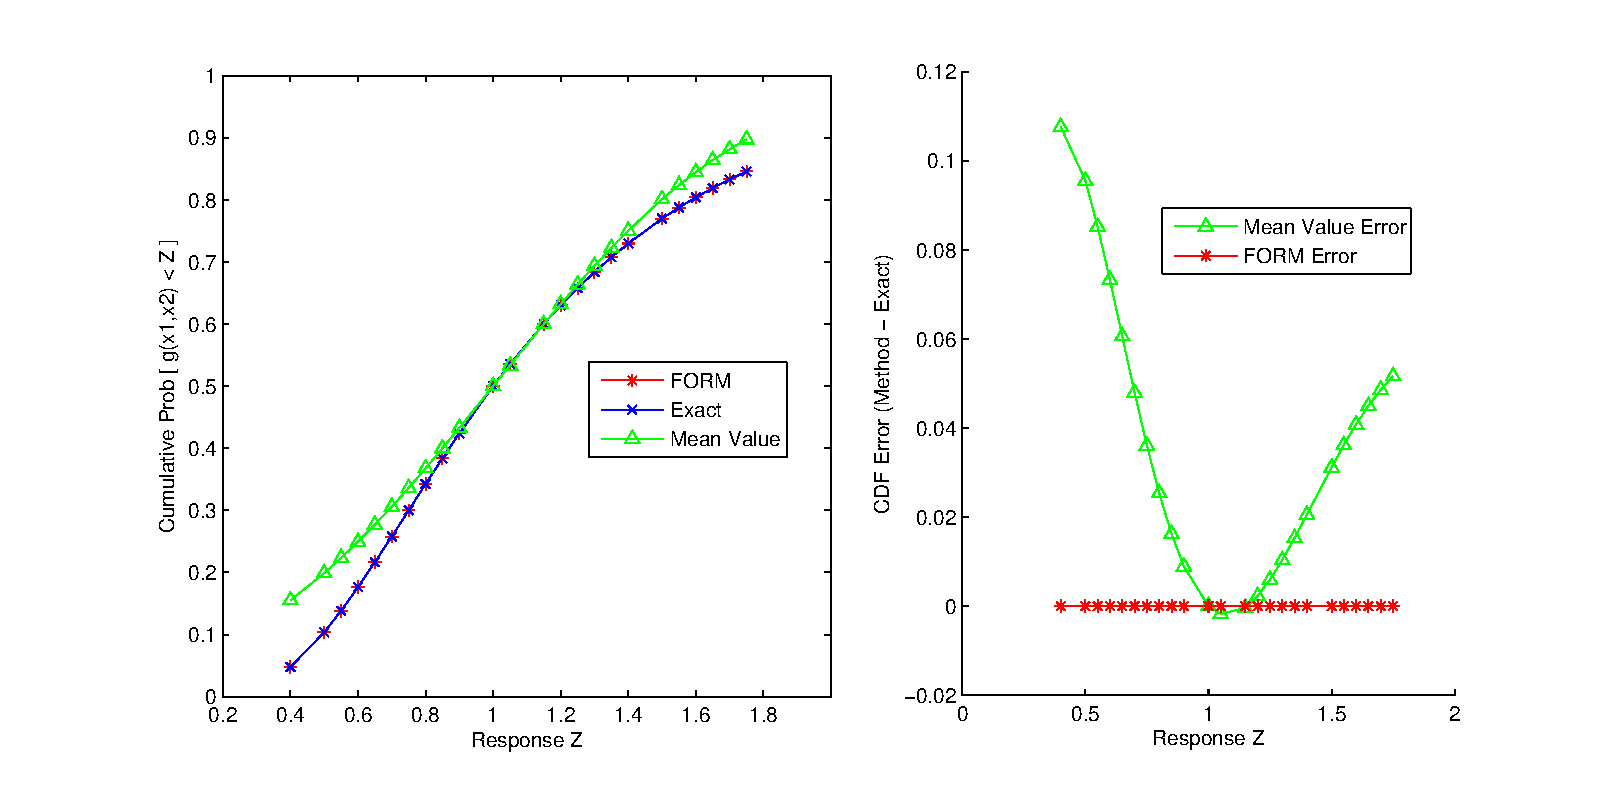
\includegraphics[scale=0.5]{images/cdf_form}
\caption{Comparison of the cumulative distribution function (CDF) computed by
FORM, the Mean Value method, and the exact CDF for $g(x_1,x_2)=\frac{x_1}{x_2}$}
\label{uq:rel_form_compare}
\end{figure}

If the user specifies \texttt{local\_reliability} as a method 
with no additional specification on how to do the MPP search, then no 
MPP search is done: the Mean Value method is used.  The MV results are
shown in Figure~\ref{uq:rel_output_mv} and consist of approximate mean
and standard deviation of the response, the importance factors for
each uncertain variable, and approximate probability/reliability
levels for the prescribed response levels that have been inferred from
the approximate mean and standard deviation (using
Equations~\ref{eq:mv_ria_cdf} and~\ref{eq:p_cdf}). It is evident that
the statistics are considerably different from the fully converged
FORM results; however, these rough approximations are also much less
expensive to calculate. The importance factors are a measure of the
sensitivity of the response function(s) to the uncertain input
variables, but in this case, are not separable due to the presence of
input correlation coefficients. A comparison of the mean value results 
with the FORM results is shown in Figure~\ref{uq:rel_form_compare}. 
The mean value results are not accurate near the tail values of the CDF, 
and can differ from the exact solution by as much as 0.11 in CDF estimates.
A comprehensive comparison of
various reliability methods applied to the logratio problem 
is provided in ~\cite{Eld06a}.

\begin{figure} % Imp factors only if uncorrelated
\begin{bigbox}
\begin{small}
\begin{verbatim}
MV Statistics for response_fn_1:
  Approximate Mean Response                  =  1.0000000000e+00
  Approximate Standard Deviation of Response =  5.9160798127e-01
  Importance Factors not available.
Cumulative Distribution Function (CDF) for response_fn_1:
     Response Level  Probability Level  Reliability Index
     --------------  -----------------  -----------------
   4.0000000000e-01   1.5524721837e-01   1.0141851006e+00
   5.0000000000e-01   1.9901236093e-01   8.4515425050e-01
   5.5000000000e-01   2.2343641149e-01   7.6063882545e-01
   6.0000000000e-01   2.4948115037e-01   6.7612340040e-01
   6.5000000000e-01   2.7705656603e-01   5.9160797535e-01
   7.0000000000e-01   3.0604494093e-01   5.0709255030e-01
   7.5000000000e-01   3.3630190949e-01   4.2257712525e-01
   8.0000000000e-01   3.6765834596e-01   3.3806170020e-01
   8.5000000000e-01   3.9992305332e-01   2.5354627515e-01
   9.0000000000e-01   4.3288618783e-01   1.6903085010e-01
   1.0000000000e+00   5.0000000000e-01   0.0000000000e+00
   1.0500000000e+00   5.3367668035e-01  -8.4515425050e-02
   1.1500000000e+00   6.0007694668e-01  -2.5354627515e-01
   1.2000000000e+00   6.3234165404e-01  -3.3806170020e-01
   1.2500000000e+00   6.6369809051e-01  -4.2257712525e-01
   1.3000000000e+00   6.9395505907e-01  -5.0709255030e-01
   1.3500000000e+00   7.2294343397e-01  -5.9160797535e-01
   1.4000000000e+00   7.5051884963e-01  -6.7612340040e-01
   1.5000000000e+00   8.0098763907e-01  -8.4515425050e-01
   1.5500000000e+00   8.2372893005e-01  -9.2966967555e-01
   1.6000000000e+00   8.4475278163e-01  -1.0141851006e+00
   1.6500000000e+00   8.6405064339e-01  -1.0987005257e+00
   1.7000000000e+00   8.8163821351e-01  -1.1832159507e+00
   1.7500000000e+00   8.9755305196e-01  -1.2677313758e+00
\end{verbatim}
\end{small}
\end{bigbox}
\caption{Output from Reliability UQ example using MV.}
\label{uq:rel_output_mv}
\end{figure}

Additional reliability analysis and design results are provided in 
Sections~\ref{additional:logratio}-\ref{additional:steel_column}.


\section{Stochastic Expansion Methods}\label{uq:expansion}


The objective of these techniques is to characterize the response of
systems whose governing equations involve stochastic coefficients. The
development of these techniques mirrors that of deterministic finite
element analysis through the utilization of the concepts of
projection, orthogonality, and weak convergence. The polynomial chaos
expansion is based on a multidimensional orthogonal polynomial
approximation in standardized random variables, and the stochastic
collocation approach is based on a multidimensional Lagrange
interpolation in standardized random variables.  A distinguishing
feature of these methodologies is that the final solution is expressed as
a random process, and not merely as a set of statistics as is the case
for many nondeterministic methodologies.  This makes these techniques
particularly attractive for use in multi-physics applications which
link different analysis packages.

The first stochastic expansion method is the polynomial chaos
expansion (PCE) described in Ghanem, et
al.~\cite{Gha99},~\cite{Gha91}.  For smooth functions (i.e., analytic,
infinitely-differentiable) in $L^2$ (i.e., possessing finite
variance), exponential convergence rates can be obtained under order
refinement for integrated statistical quantities of interest such as
mean, variance, and probability.  DAKOTA implements the generalized
polynomial chaos approach using the Wiener-Askey
scheme~\cite{XiuKarn02}, in which Hermite, Legendre, Laguerre, Jacobi,
and generalized Laguerre orthogonal polynomials are used for modeling
the effect of continuous random variables described by normal,
uniform, exponential, beta, and gamma probability distributions,
respectively\footnote{Orthogonal polynomial selections also exist for
discrete probability distributions, but are not yet supported in
DAKOTA.}.  These orthogonal polynomial selections are optimal for
these distribution types since the inner product weighting function
corresponds\footnote{Identical support range; weight
differs by at most a constant factor.} to the probability
density functions for these continuous distributions.  Orthogonal polynomials
can be computed for any positive weight function, so these five
classical orthogonal polynomials may be augmented with
numerically-generated polynomials for other probability distributions
(e.g., for lognormal, extreme value, and histogram distributions).
When independent standard random variables are used (or computed
through transformation), the variable expansions are uncoupled,
allowing the polynomial orthogonality properties to be applied on a
per-dimension basis.  This allows one to mix and match the polynomial
basis used for each variable without interference with the spectral
projection scheme for the response.  

In non-intrusive PCE, simulations are used as black boxes and the
calculation of chaos expansion coefficients for response metrics of
interest is based on a set of simulation response evaluations.  To
calculate these response PCE coefficients, two primary classes of
approaches have been proposed: spectral projection and linear
regression.  The spectral projection approach projects the response
against each basis function using inner products and employs the
polynomial orthogonality properties to extract each coefficient.  Each
inner product involves a multidimensional integral over the support
range of the weighting function, which can be evaluated numerically
using sampling, tensor-product quadrature, Smolyak sparse
grid~\cite{Smolyak_63}, or cubature~\cite{stroud} approaches.  The
linear regression approach uses a single linear least squares solution
to solve for the set of PCE coefficients which best match a set of
response values obtained from either a design of computer experiments
(``point collocation''~\cite{pt_colloc1}) or from the subset of tensor
Gauss points with highest product weight (``probabilistic
collocation''~\cite{Tat95}).

Stochastic collocation (SC) is another stochastic expansion technique
for UQ that is closely related to PCE.  As for PCE,
exponential convergence rates can be obtained under order refinement
for integrated statistical quantities of interest, provided that the
response functions are smooth with finite variance.  The primary
distinction is that, whereas PCE estimates coefficients for known
orthogonal polynomial basis functions, SC forms Lagrange interpolation
functions for known coefficients.  
Interpolation is performed on structured grids such as tensor-product
or sparse grids.  Starting from a tensor-product multidimensional
Lagrange interpolant, we have the feature that the $i^{th}$
interpolation polynomial is 1 at collocation point $i$ and 0 for all
other collocation points, leading to the use of expansion coefficients
that are just the response values at each of the collocation points.
Sparse interpolants are weighted sums of these tensor interpolants;
%and retain the use of response values as expansion coefficients;
however, they are only interpolatory for sparse grids based on fully 
nested rules and will exhibit some interpolation error at the 
collocation points for sparse grids based on non-nested rules.
A key to maximizing performance with SC is performing collocation
using the Gauss points and weights from the same optimal orthogonal
polynomials used in PCE.  
For use of standard Gauss integration rules (not nested variants such
as Gauss-Patterson or Genz-Keister) within tensor-product quadrature,
tensor PCE expansions and tensor SC interpolants are equivalent in
that identical polynomial approximations are
generated~\cite{ConstTPQ}.  Moreover, this equivalence can be extended
to sparse grids based on standard Gauss rules, provided that a sparse
PCE is formed based on a weighted sum of tensor expansions~\cite{ConstSSG}.


\subsection{Orthogonal polynomials in the Askey scheme} \label{uq:expansion:askey}

Table~\ref{TAB:askey} shows the set of classical orthogonal
polynomials which provide an optimal basis for different continuous
probability distribution types.  It is derived from the family of
hypergeometric orthogonal polynomials known as the Askey
scheme~\cite{askey}, for which the Hermite polynomials originally
employed by Wiener~\cite{wiener} are a subset.  The optimality of
these basis selections derives from their orthogonality with respect
to weighting functions that correspond to the probability density
functions (PDFs) of the continuous distributions when placed in a
standard form.  The density and weighting functions differ by a
constant factor due to the requirement that the integral of the PDF
over the support range is one.

\begin{table}[h]
  \centering
  \caption{Linkage between standard forms of continuous probability distributions and Askey scheme of continuous hyper-geometric polynomials.}
  \label{TAB:askey} 
  \begin{tabular}{ccccc} \hline
   Distribution & Density function & Polynomial & Weight function & Support range \\ \hline \hline
   Normal      & $\frac{1}{\sqrt{2\pi}} e^{\frac{-x^2}{2}}$ & Hermite  $He_n(x)$ & $e^{\frac{-x^2}{2}}$ & $[-\infty, \infty]$ \\ \hline
   Uniform     & $\frac{1}{2}$ & Legendre $P_n(x)$ & $1$ & $[-1,1]$ \\ \hline
   Beta        & $ \frac{(1-x)^{\alpha}(1+x)^{\beta}}{2^{\alpha+\beta+1} B(\alpha+1,\beta+1)}$ & Jacobi   $P^{(\alpha,\beta)}_n(x)$ & $(1-x)^{\alpha}(1+x)^{\beta}$ & $[-1,1]$ \\ \hline
   Exponential & $e^{-x}$ & Laguerre $L_n(x)$ & $e^{-x}$ & $[0, \infty]$ \\ \hline
   Gamma       & $\frac{x^{\alpha} e^{-x}}{\Gamma(\alpha+1)}$ & Generalized Laguerre $L^{(\alpha)}_n(x)$ & $x^{\alpha} e^{-x}$ & $[0, \infty]$ \\ \hline \hline
  \end{tabular}
\end{table}

Note that Legendre is a special case of Jacobi for 
$\alpha = \beta = 0$, Laguerre is a special case of generalized 
Laguerre for $\alpha = 0$, $\Gamma(a)$ is the Gamma function which 
extends the factorial function to continuous values, and $B(a,b)$ is the 
Beta function defined as $B(a,b) = \frac{\Gamma(a)\Gamma(b)}{\Gamma(a+b)}$.
Some care is necessary when specifying the $\alpha$ and $\beta$
parameters for the Jacobi and generalized Laguerre polynomials since
the orthogonal polynomial conventions~\cite{abram_stegun} differ from
the common statistical PDF conventions.  The former conventions are
used in Table~\ref{TAB:askey}.

\subsection{Numerically generated orthogonal polynomials} 
\label{uq:expansion:beyond_askey}

If all random inputs can be described using independent normal, 
uniform, exponential, beta, and gamma distributions, then Askey 
polynomials can be directly applied.  If correlation or other distribution
types are present, then additional techniques are required.  One
solution is to employ nonlinear variable transformations as described
in Section~\ref{uq:expansion:trans} such that an Askey basis can be 
applied in the transformed space.  This can be effective as shown
in~\cite{Eld07}, but convergence rates are typically degraded.  In
addition, correlation coefficients are warped by the nonlinear
transformation~\cite{Der86}, and simple expressions for these
transformed correlation values are not always readily available.  An
alternative is to numerically generate the orthogonal polynomials
(using Gauss-Wigert~\cite{simpson_gw}, discretized
Stieltjes~\cite{gautschi_book}, Chebyshev~\cite{gautschi_book}, or
Gramm-Schmidt~\cite{WillBijl06} approaches) and then compute their
Gauss points and weights (using the Golub-Welsch~\cite{GolubWelsch69}
tridiagonal eigensolution).  These solutions are optimal for given
random variable sets having arbitrary probability density functions and 
%preserve the exponential convergence rates for general UQ applications,
%and also eliminates the need to calculate correlation warping.
eliminate the need to induce additional nonlinearity through variable
transformations, but performing this process for general joint density
functions with correlation is a topic of ongoing research (refer to
Section~\ref{uq:expansion:trans} for additional details).

\subsection{Interpolation polynomials} \label{uq:expansion:interp}

Lagrange polynomials interpolate a set of points in a single dimension
using the functional form
\begin{equation}
L_j = \prod_{\stackrel{\scriptstyle k=1}{k \ne j}}^m 
\frac{\xi - \xi_k}{\xi_j - \xi_k} \label{eq:lagrange_poly_1d}
\end{equation}
where it is evident that $L_j$ is 1 at $\xi = \xi_j$, is 0 for each of
the points $\xi = \xi_k$, and has order $m - 1$.

For interpolation of a response function $R$ in one dimension over $m$
points, the expression
\begin{equation}
R(\xi) \cong \sum_{j=1}^m r(\xi_j)\,L_j(\xi) \label{eq:lagrange_interp_1d}
\end{equation}
reproduces the response values $r(\xi_j)$ at the interpolation points
and smoothly interpolates between these values at other points.  For
interpolation in multiple dimensions, a tensor-product approach is
used wherein
\begin{equation}
R(\boldsymbol{\xi}) \cong \sum_{j_1=1}^{m_{i_1}}\cdots\sum_{j_n=1}^{m_{i_n}}
r\left(\xi^{i_1}_{j_1},\dots , \xi^{i_n}_{j_n}\right)\,
\left(L^{i_1}_{j_1}\otimes\cdots\otimes L^{i_n}_{j_n}\right)
= \sum_{j=1}^{N_p} r_j(\boldsymbol{\xi}) \boldsymbol{L}_j(\boldsymbol{\xi})
\label{eq:lagrange_interp_nd}
\end{equation}
where $\boldsymbol{i} = (m_1, m_2, \cdots, m_n)$ are the number of
nodes used in the $n$-dimensional interpolation and $\xi^i_j$ is the
$j$-th point in the $i$-th direction.  As will be seen later,
interpolation on sparse grids involves a summation of these tensor
products with varying $\boldsymbol{i}$ levels.


\subsection{Generalized Polynomial Chaos} \label{uq:expansion:pce}

The set of polynomials from \ref{uq:expansion:askey}
and~\ref{uq:expansion:beyond_askey} are used as an orthogonal basis to
approximate the functional form between the stochastic response output
and each of its random inputs.  The chaos expansion for a response $R$
takes the form
\begin{equation}
R = a_0 B_0 + \sum_{i_1=1}^{\infty} a_{i_1} B_1(\xi_{i_1}) + 
\sum_{i_1=1}^{\infty} \sum_{i_2=1}^{i_1} a_{i_1i_2} B_2(\xi_{i_1},\xi_{i_2}) +
\sum_{i_1=1}^{\infty} \sum_{i_2=1}^{i_1} \sum_{i_3=1}^{i_2} a_{i_1i_2i_3}
B_3(\xi_{i_1},\xi_{i_2},\xi_{i_3}) + ...\label{eq:expansion_long}
\end{equation}
where the random vector dimension is unbounded and each additional set
of nested summations indicates an additional order of polynomials in
the expansion.  This expression can be simplified by replacing the
order-based indexing with a term-based indexing
\begin{equation}
R = \sum_{j=0}^{\infty} \alpha_j \Psi_j(\boldsymbol{\xi})
\label{eq:expansion_short}
\end{equation}
where there is a one-to-one correspondence between $a_{i_1i_2...i_n}$
and $\alpha_j$ and between
$B_n(\xi_{i_1},\xi_{i_2},...,\xi_{i_n})$ and
$\Psi_j(\boldsymbol{\xi})$.  Each of the
$\Psi_j(\boldsymbol{\xi})$ are multivariate polynomials
which involve products of the one-dimensional polynomials.  For
example, a multivariate Hermite polynomial
$B(\boldsymbol{\xi})$ of order $n$ is defined from
\begin{equation}
B_n(\xi_{i_1}, ..., \xi_{i_n}) = 
e^{\frac{1}{2}\boldsymbol{\xi}^T\boldsymbol{\xi}} (-1)^n 
\frac{\partial^n}{\partial \xi_{i_1} ... \partial \xi_{i_n}} 
e^{-\frac{1}{2}\boldsymbol{\xi}^T\boldsymbol{\xi}} \label{eq:multivar_gen}
\end{equation}
which can be shown to be a product of one-dimensional Hermite polynomials
involving a multi-index $m_i^j$:
\begin{equation}
B_n(\xi_{i_1}, ..., \xi_{i_n}) = 
\Psi_j(\boldsymbol{\xi}) = 
\prod_{i=1}^{n} \psi_{m_i^j}(\xi_i) \label{eq:multivar_prod}
\end{equation}
%which provides a convenient form for sensitivity analysis as described
%in \ref{uq:expansion:rvsa}.
In the case of a mixed basis, the same multi-index definition is
employed although the one-dimensional polynomials $\psi_{m_i^j}$ are
heterogeneous in type.

\subsubsection{Expansion truncation and tailoring} \label{uq:expansion:pce:exp_tnt}

In practice, one truncates the infinite expansion at a finite number
of random variables and a finite expansion order
\begin{equation}
R \cong \sum_{j=0}^P \alpha_j \Psi_j(\boldsymbol{\xi})
\label{eq:pc_exp_trunc}
\end{equation}
Traditionally, the polynomial chaos expansion includes a complete
basis of polynomials up to a fixed total-order specification.  That is,
for an expansion of total order $p$ involving $n$ random variables, the 
multi-index defining the set of $\Psi_j$ is constrained by
\begin{equation}
\sum_{i=1}^{n} m_i^j \leq p \label{eq:to_multi_index}
\end{equation}
For example, the multidimensional basis polynomials for a second-order
expansion over two random dimensions are
\begin{eqnarray}
\Psi_0(\boldsymbol{\xi}) & = & \psi_0(\xi_1) ~ \psi_0(\xi_2) ~~=~~ 1 
\nonumber \\
\Psi_1(\boldsymbol{\xi}) & = & \psi_1(\xi_1) ~ \psi_0(\xi_2) ~~=~~ \xi_1 
\nonumber \\
\Psi_2(\boldsymbol{\xi}) & = & \psi_0(\xi_1) ~ \psi_1(\xi_2) ~~=~~ \xi_2 
\nonumber \\
\Psi_3(\boldsymbol{\xi}) & = & \psi_2(\xi_1) ~ \psi_0(\xi_2) ~~=~~ \xi_1^2 - 1 
\nonumber \\
\Psi_4(\boldsymbol{\xi}) & = & \psi_1(\xi_1) ~ \psi_1(\xi_2) ~~=~~ \xi_1 \xi_2 
\nonumber \\
\Psi_5(\boldsymbol{\xi}) & = & \psi_0(\xi_1) ~ \psi_2(\xi_2) ~~=~~ \xi_2^2 - 1 
\nonumber 
\end{eqnarray}
The total number of terms $N_t$ in an expansion of total order
$p$ involving $n$ random variables is given by
\begin{equation}
N_t ~=~ 1 + P ~=~ 1 + \sum_{s=1}^{p} {\frac{1}{s!}} \prod_{r=0}^{s-1} (n+r)
    ~=~ \frac{(n+p)!}{n!p!} \label{eq:num_to_terms}
\end{equation}
This traditional approach will be referred to as a ``total-order
expansion.''

An important alternative approach is to employ a ``tensor-product
expansion,'' in which polynomial order bounds are applied on a
per-dimension basis (no total-order bound is enforced) and all
combinations of the one-dimensional polynomials are included.  That 
is, the multi-index defining the set of $\Psi_j$ is constrained by
\begin{equation}
m_i^j \leq p_i \label{eq:tp_multi_index}
\end{equation}
where $p_i$ is the polynomial order bound for the $i$-th dimension.
In this case, the example basis for $p = 2, n = 2$ is
\begin{eqnarray}
\Psi_0(\boldsymbol{\xi}) & = & \psi_0(\xi_1) ~ \psi_0(\xi_2) ~~=~~ 1 
\nonumber \\
\Psi_1(\boldsymbol{\xi}) & = & \psi_1(\xi_1) ~ \psi_0(\xi_2) ~~=~~ \xi_1 
\nonumber \\
\Psi_2(\boldsymbol{\xi}) & = & \psi_2(\xi_1) ~ \psi_0(\xi_2) ~~=~~ \xi_1^2 - 1
\nonumber \\
\Psi_3(\boldsymbol{\xi}) & = & \psi_0(\xi_1) ~ \psi_1(\xi_2) ~~=~~ \xi_2
\nonumber \\
\Psi_4(\boldsymbol{\xi}) & = & \psi_1(\xi_1) ~ \psi_1(\xi_2) ~~=~~ \xi_1 \xi_2 
\nonumber \\
\Psi_5(\boldsymbol{\xi}) & = & \psi_2(\xi_1) ~ \psi_1(\xi_2) ~~=~~ 
(\xi_1^2 - 1) \xi_2 \nonumber \\
\Psi_6(\boldsymbol{\xi}) & = & \psi_0(\xi_1) ~ \psi_2(\xi_2) ~~=~~ \xi_2^2 - 1 
\nonumber \\
\Psi_7(\boldsymbol{\xi}) & = & \psi_1(\xi_1) ~ \psi_2(\xi_2) ~~=~~ 
\xi_1 (\xi_2^2 - 1) \nonumber \\
\Psi_8(\boldsymbol{\xi}) & = & \psi_2(\xi_1) ~ \psi_2(\xi_2) ~~=~~ 
(\xi_1^2 - 1) (\xi_2^2 - 1) \nonumber
\end{eqnarray}
and the total number of terms $N_t$ is
\begin{equation}
N_t ~=~ 1 + P ~=~ \prod_{i=1}^{n} (p_i + 1) \label{eq:num_tp_terms}
\end{equation}

It is apparent from Eq.~\ref{eq:num_tp_terms} that the tensor-product
expansion readily supports anisotropy in polynomial order for each
dimension, since the polynomial order bounds for each dimension can be
specified independently.  It is also feasible to support anisotropy
with total-order expansions, through pruning polynomials that satisfy 
the total-order bound 
%(potentially defined from the maximum of the per-dimension bounds)
but violate individual per-dimension bounds (the number of these
pruned polynomials would then be subtracted from
Eq.~\ref{eq:num_to_terms}).  Finally, custom tailoring of the
expansion form can also be explored, e.g. to closely synchronize with
monomial coverage in sparse grids through use of a summation of tensor
expansions (see Section~\ref{uq:expansion:spectral_sparse}).
%Of particular interest is the tailoring of expansion form to target
%specific monomial coverage as motivated by the integration process
%employed for evaluating chaos coefficients.  If the specific monomial
%set that can be resolved by a particular integration approach is known
%or can be approximated, then the chaos expansion can be tailored to
%synchonize with this set.  Tensor-product and total-order expansions
%can be seen as special cases of this general approach (corresponding
%to tensor-product quadrature and Smolyak sparse grids with linear
%growth rules, respectively), whereas, for example, Smolyak sparse
%grids with nonlinear growth rules could generate synchonized expansion
%forms that are neither tensor-product nor total-order (to be discussed
%later in association with Figure~\ref{fig:pascal_sparse_lev4_Gauss}).
In all cases, the specifics of the expansion are codified in the
multi-index, and subsequent machinery for estimating response values
and statistics from the expansion
%(estimating response values at particular $\boldsymbol{\xi}$, evaluating
%response statistics by integrating over $\boldsymbol{\xi}$, etc.)
can be performed in a manner that is agnostic to the specific 
expansion form.


\subsection{Stochastic Collocation} \label{uq:expansion:sc}

The SC expansion is formed as a sum of a set of multidimensional
Lagrange interpolation polynomials, one polynomial per unique
collocation point.  Since these polynomials have the feature of being
equal to 1 at their particular collocation point and 0 at all other
points\footnote{for tensor interpolants and sparse interpolants based
on fully nested rules (e.g., Clenshaw-Curtis, Gauss-Patterson,
Genz-Keister); sparse interpolants based on non-nested rules will
exhibit some interpolation error at the collocation points}, the
coefficients of the expansion are just the response values at each of
the collocation points.  This can be written as:
\begin{equation}
R \cong \sum_{j=1}^{N_p} r_j \boldsymbol{L}_j(\boldsymbol{\xi}) 
\label{eq:sc_exp_short}
\end{equation}
where the set of $N_p$ collocation points involves a structured
multidimensional grid (a tensor-product grid as in
Eq.~\ref{eq:lagrange_interp_nd} or a Smolyak sparse grid).  There is
no need for tailoring of the expansion form as there is for PCE (i.e.,
to synchronize the expansion polynomials with the set of integrable
monomials) since the polynomials that appear in the expansion are
determined by the Lagrange construction
(Eq.~\ref{eq:lagrange_poly_1d}).  That is, any tailoring or refinement
of the expansion occurs through the selection of points in the
interpolation grid and the polynomial orders of the basis are adapted
implicitly.


\subsection{Transformations to uncorrelated standard variables} \label{uq:expansion:trans}

Polynomial chaos and stochastic collocation are expanded using
polynomials that are functions of independent standard random
variables $\boldsymbol{\xi}$.  Thus, a key component of either
approach is performing a transformation of variables from the original
random variables $\boldsymbol{x}$ to independent standard random
variables $\boldsymbol{\xi}$ and then applying the stochastic
expansion in the transformed space.  %The dimension of
%$\boldsymbol{\xi}$ is typically chosen to correspond to the dimension
%of $\boldsymbol{x}$, although this is not required.  In fact, the
%dimension of $\boldsymbol{\xi}$ should be chosen to represent the
%number of distinct sources of randomness in a particular problem, and
%if individual $x_i$ mask multiple random inputs, then the dimension of
%$\boldsymbol{\xi}$ can be expanded to accommodate~\cite{ghanem_private}.
%For simplicity, all subsequent discussion will assume a one-to-one 
%correspondence between $\boldsymbol{\xi}$ and $\boldsymbol{x}$.
This notion of independent standard space is extended over the notion
of ``u-space'' used in reliability methods (see
Section~\ref{uq:reliability:mpp}) 
in that it extends the standardized set beyond standard normals.
%includes not just independent standard normals, but also independent 
%standard uniforms, exponentials, betas, and gammas.
%For problems directly involving independent input distributions of
%these five types, conversion to standard form involves a simple linear
%scaling transformation (to the form of the density functions in
%Table~\ref{TAB:askey}) and then the corresponding chaos/collocation
%points can be employed.  For correlated normal,
%uniform, exponential, beta, and gamma distributions, the same linear
%scaling transformation can be applied followed by application of the
%inverse Cholesky factor of the correlation matrix (similar to
%Eq.~\ref{eq:trans_zu} below, but the correlation matrix requires no
%modification for linear transformations).  As described previously,
%the subsequent independence assumption is valid for uncorrelated
%standard normals but may introduce significant error for other random
%variable types (this is currently a topic of ongoing research).  
For distributions that are already independent, three different 
approaches are of interest:
%one has a choice of up to three different approaches, depending on
%the types of distributions that are present:
\begin{enumerate}
\item {\it Extended basis:} For each Askey distribution type, employ
  the corresponding Askey basis (Table~\ref{TAB:askey}).  For
  non-Askey types, numerically generate an optimal polynomial basis
  for each independent distribution as described in
  Section~\ref{uq:expansion:beyond_askey}.
  % text below moved downstream from Intro:
  With usage of the optimal basis corresponding to each of the random
  variable types, we can exploit basis orthogonality under expectation
  (e.g., Eq.~\ref{eq:coeff_extract}) without requiring a transformation
  of variables, thereby avoiding inducing additional nonlinearity that
  could slow convergence.
\item {\it Askey basis:} For non-Askey types, perform a nonlinear
  variable transformation from a given input distribution to the most
  similar Askey basis.  For example, lognormal distributions might
  employ a Hermite basis in a transformed standard normal space and
  loguniform, triangular, and histogram distributions might employ a
  Legendre basis in a transformed standard uniform space.  All
  distributions then employ the Askey orthogonal polynomials and
  their associated Gauss points/weights.
\item {\it Wiener basis:} For non-normal distributions, employ a
  nonlinear variable transformation to standard normal distributions. All
  distributions then employ the Hermite orthogonal polynomials and
  their associated Gauss points/weights.
\end{enumerate}
For dependent distributions, we must first perform a nonlinear
variable transformation to uncorrelated standard normal distributions,
due to the independence of decorrelated standard normals.  This
involves the Nataf transformation, described in the following
paragraph.  We then have the following choices:
\begin{enumerate}
%\setcounter{enumi}{2}
\item {\it Single transformation:} Following the Nataf transformation
  to independent standard normal distributions, employ the Wiener
  basis in the transformed space.
\item {\it Double transformation:} From independent standard normal
  space, transform back to either the original marginal distributions
  or the desired Askey marginal distributions and employ an extended
  or Askey basis, respectively, in the transformed space. Independence
  is maintained, but the nonlinearity of the Nataf transformation is
  at least partially mitigated.
  % Note: no secondary warping since no correlation.
\end{enumerate}
DAKOTA currently supports single transformations for dependent
variables in combination with an Askey basis for independent variables.

The transformation from correlated non-normal distributions to
uncorrelated standard normal distributions is denoted as
$\boldsymbol{\xi} = T({\bf x})$ with the reverse transformation denoted as
${\bf x} = T^{-1}(\boldsymbol{\xi})$.  These transformations are nonlinear in
general, and possible approaches include the Rosenblatt~\cite{Ros52},
Nataf~\cite{Der86}, and Box-Cox~\cite{Box64} transformations.
%The nonlinear transformations may also be linearized, and common
%approaches for this include the Rackwitz-Fiessler~\cite{rf}
%two-parameter equivalent normal and the Chen-Lind~\cite{cl} and
%Wu-Wirsching~\cite{ww} three-parameter equivalent normals.
The results in this paper employ the Nataf transformation,
which is suitable for the common case when marginal distributions and
a correlation matrix are provided, but full joint distributions are
not known\footnote{If joint distributions are known, then the
Rosenblatt transformation is preferred.}.  The Nataf transformation
occurs in the following two steps.  To transform between the original
correlated x-space variables and correlated standard normals
(``z-space''), a CDF matching condition is applied for each of the
marginal distributions:
\begin{equation}
\Phi(z_i) = F(x_i) %\label{eq:trans_zx}
\end{equation}
where $\Phi()$ is the standard normal cumulative distribution function
and $F()$ is the cumulative distribution function of the original
probability distribution.  Then, to transform between correlated
z-space variables and uncorrelated $\xi$-space variables, the Cholesky
factor ${\bf L}$ of a modified correlation matrix is used:
\begin{equation}
{\bf z} = {\bf L} \boldsymbol{\xi} %\label{eq:trans_zu}
\end{equation}
where the original correlation matrix for non-normals in x-space has
been modified to represent the corresponding ``warped'' correlation in
z-space~\cite{Der86}.


\subsection{Spectral projection} \label{uq:expansion:spectral}

The major practical difference between PCE and SC is that, in PCE, one
must estimate the coefficients for known basis functions, whereas in
SC, one must form the interpolants for known coefficients.  PCE
estimates its coefficients using either spectral projection or linear
regression, where the former approach involves numerical integration
based on random sampling, tensor-product quadrature, Smolyak sparse
grids, or cubature methods.  In SC, the multidimensional interpolants
need to be formed over structured data sets, such as point sets from
quadrature or sparse grids; approaches based on random sampling may
not be used.  

The spectral projection approach
%(which justifies the term stochastic finite elements)
projects the response against each basis function using inner products
and employs the polynomial orthogonality properties to extract each
coefficient.  Similar to a Galerkin projection, the residual error
from the approximation is rendered orthogonal to the selected basis.
From Eq.~\ref{eq:pc_exp_trunc}, taking the inner product of both sides
with respect to $\Psi_j$ and enforcing orthogonality yields:
\begin{equation}
\alpha_j ~=~ \frac{\langle R, \Psi_j \rangle}{\langle \Psi^2_j \rangle}
~=~ {1\over {\langle \Psi^2_j \rangle}}
 \int_{\Omega} R\, \Psi_j\, \varrho(\boldsymbol{\xi}) \,d\boldsymbol{\xi},
\label{eq:coeff_extract}
\end{equation}
where each inner product involves a multidimensional integral over
the support range of the weighting function.  In particular, 
$\Omega = \Omega_1\otimes\dots\otimes\Omega_n$, with possibly
unbounded intervals $\Omega_j\subset\mathbb{R}$ and the tensor product 
form $\varrho(\boldsymbol{\xi}) = \prod_{i=1}^n \varrho_i(\xi_i)$ 
of the joint probability density (weight) function.  The denominator 
in Eq.~\ref{eq:coeff_extract} is the norm squared of the multivariate
orthogonal polynomial, which can be computed analytically using the
product of univariate norms squared
\begin{equation}
\langle \Psi^2_j \rangle ~=~ \prod_{i=1}^{n} \langle \psi_{m_i^j}^2 \rangle
\label{eq:norm_squared}
\end{equation}
where the univariate inner products have simple closed form
expressions for each polynomial in the Askey
scheme~\cite{abram_stegun} and are readily computed as part of the
numerically-generated solution procedures described in
Section~\ref{uq:expansion:beyond_askey}. Thus, the primary
computational effort resides in evaluating the numerator, which is
evaluated numerically using sampling, quadrature, cubature, or sparse
grid approaches (and this numerical approximation leads to use of the
term ``pseudo-spectral'' by some investigators).


\subsubsection{Sampling} \label{uq:expansion:spectral_samp}

In the sampling approach, the integral evaluation is equivalent to
computing the expectation (mean) of the response-basis function
product (the numerator in Eq.~\ref{eq:coeff_extract}) for each term in
the expansion when sampling within the density of the weighting
function.  This approach is only valid for PCE and since sampling does
not provide any particular monomial coverage guarantee, it is common
to combine this coefficient estimation approach with a total-order
chaos expansion.

In computational practice, coefficient estimations based on sampling
benefit from first estimating the response mean (the first PCE
coefficient) and then removing the mean from the expectation
evaluations for all subsequent coefficients.  While this has no effect
for quadrature/sparse grid methods (see following two sections) and
little effect for fully-resolved sampling, it does have a small but
noticeable beneficial effect for under-resolved sampling.


\subsubsection{Tensor product quadrature} \label{uq:expansion:spectral_quad}

In quadrature-based approaches, the simplest general technique for
approximating multidimensional integrals, as in
Eq.~\ref{eq:coeff_extract}, is to employ a tensor product of
one-dimensional quadrature rules.  %In the case where $\Omega$ is a
%hypercube, i.e. $\Omega=[-1,1]^n$, there are several choices of nested
%abscissas, included Clenshaw-Curtis, Gauss-Patterson,
%etc.~\cite{webster1, webster2, gerstner_griebel_98}.  
Since there is little benefit to the use of nested quadrature rules in
the tensor-product case\footnote{Unless a refinement procedure is in
  use.}, we choose Gaussian abscissas, i.e. the zeros of polynomials
that are orthogonal with respect to a density function weighting,
e.g. Gauss-Hermite, Gauss-Legendre, Gauss-Laguerre, generalized
Gauss-Laguerre, Gauss-Jacobi, or numerically-generated Gauss rules.

We first introduce an index $i\in\mathbb{N}_+$, $i\ge1$. Then, for
each value of $i$, let $\{\xi_1^i, \ldots,\xi_{m_i}^i\}\subset \Omega_i$ 
be a sequence of abscissas for quadrature on $\Omega_i$.  For 
$f\in C^0(\Omega_i)$ and $n=1$ we introduce a sequence of
one-dimensional quadrature operators
%$\mathscr{U}^i:\, C^0(\Gamma^1; W(D))\rightarrow V_{m_i}(\Gamma^1; W(D))$
\begin{equation}\label{eq:1d_quad}
\mathscr{U}^i(f)(\xi)=\sum_{j=1}^{m_i}f(\xi_j^i)\, w^i_j, 
%\quad\forall u\in C^0(\Gamma^1; W(D)),
\end{equation}
with $m_i\in\mathbb{N}$ given.  When utilizing Gaussian quadrature,
Eq.~\ref{eq:1d_quad} integrates exactly all polynomials of degree less
than $2m_i -1$, for each $i=1,\ldots, n$.  Given an expansion order
$p$, the highest order coefficient evaluations
(Eq.~\ref{eq:coeff_extract}) can be assumed to involve integrands of
at least polynomial order $2p$ ($\Psi$ of order $p$ and $R$ modeled to
order $p$) in each dimension such that a minimal Gaussian quadrature
order of $p+1$ will be required to obtain good accuracy in these
coefficients.

Now, in the multivariate case $n>1$, for each $f\in C^0(\Omega)$ and
the multi-index $\mathbf{i}=(i_1,\dots,i_n)\in\mathbb{N}_+^n$ we
define the full tensor product quadrature formulas
%
\begin{equation}\label{eq:multi_tensor}
\mathcal{Q}_{\mathbf{i}}^n f(\xi)=\left(\mathscr{U}^{i_1}\otimes\cdots\otimes\mathscr{U}^{i_n}\right)(f)(\boldsymbol{\xi})=
\sum_{j_1=1}^{m_{i_1}}\cdots\sum_{j_n=1}^{m_{i_n}}
f\left(\xi^{i_1}_{j_1},\dots , \xi^{i_n}_{j_n}\right)\,\left(w^{i_1}_{j_1}\otimes\cdots\otimes w^{i_n}_{j_n}\right).
\end{equation}
Clearly, the above product needs $\prod_{j=1}^n m_{i_j}$ function
evaluations.  Therefore, when the number of input random variables is
small, full tensor product quadrature is a very effective numerical
tool.  On the other hand, approximations based on tensor product grids
suffer from the \emph{curse of dimensionality} since the number of
collocation points in a tensor grid grows exponentially fast in the
number of input random variables.  For example, if
Eq.~\ref{eq:multi_tensor} employs the same order for all random dimensions,
$m_{i_j} = m$, then Eq.~\ref{eq:multi_tensor} requires $m^n$ function
evaluations.

%Figure~\ref{fig:pascal_tensor_quad5_Gauss} depicts the monomial
%coverage in Pascal's triangle for an integrand evaluated using an
%isotropic Gaussian quadrature rules in two dimensions ($m_1 = m_2 =
%5$).  Given this type of coverage, the traditional approach of
%exploying a total-order PCE (involving integrands indicated by the red
%horizontal line) neglects a significant portion of the monomial
%coverage and one would expect a tensor-product PCE to provide improved
%synchronization and more effective usage of the Gauss point
%evaluations.  In fact, use of a tensor-expansion improves PCE
%performance significantly and has been shown to result in identical
%polynomial forms to SC~\cite{ConstTPQ}, eliminating a performance gap
%that exists in the total-order expansion case.  Note that the
%integrand monomial coverage must resolve $2p$, such that $p_1 = p_2 =
%4$ would be selected in this example (preferring slight
%over-integration to under-integration) for either the tensor or
%total-order expansion cases.
%\begin{figure}[h!]
%\begin{center}
%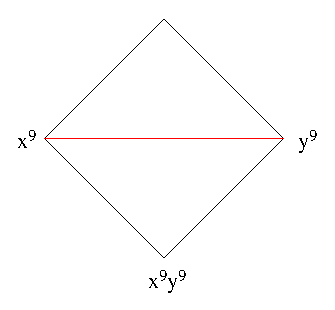
\includegraphics[width=2.5in]{TensorQuad5_Gauss}
%\caption{Pascal's triangle depiction of integrand monomial coverage 
%for two dimensions and Gaussian tensor-product quadrature order = 5.
%Red line depicts maximal total-order integrand coverage.}
%\label{fig:pascal_tensor_quad5_Gauss}
%\end{center}
%\end{figure} 

In~\cite{Eld09a}, it is demonstrated that close synchronization of
expansion form with the monomial resolution of a particular numerical
integration technique can result in significant performance
improvements.  In particular, the traditional approach of exploying a
total-order PCE (Eqs.~\ref{eq:to_multi_index}--\ref{eq:num_to_terms})
neglects a significant portion of the monomial coverage for a
tensor-product quadrature approach, and one should rather employ a
tensor-product PCE (Eqs.~\ref{eq:tp_multi_index}--\ref{eq:num_tp_terms}) 
to provide improved synchronization and more effective usage of the
Gauss point evaluations.  When the quadrature points are standard
Gauss rules (i.e., no Clenshaw-Curtis, Gauss-Patterson, or
Genz-Keister nested rules), it has been shown that tensor-product PCE
and SC result in identical polynomial forms~\cite{ConstTPQ},
completely eliminating a performance gap that exists between
total-order PCE and SC~\cite{Eld09a}.


\subsubsection{Smolyak sparse grids} \label{uq:expansion:spectral_sparse}

% For m = max points per dim, w = level:
%   Gaussian Smolyak: m = 2^(w+1) - 1  -->  m = 1, 3, 7, 15, 31, 63, 127
%   Clenshaw-Curtis:  m = 2^w     + 1  -->  m = 1, 3, 5,  9, 17, 33,  65
% TP logic would use:
%   Gaussian Smolyak: 2p <= 2m-1
%   Clenshaw-Curtis:  2p <=  m+1
% SG order selection instead using 2p <= m,
% as this is what has been observed thus far.

If the number of random variables is moderately large, one should rather
consider sparse tensor product spaces as first proposed by Smolyak
\cite{Smolyak_63} and further investigated by Refs.~\cite{gerstner_griebel_98,barth_novak_ritter_00,Fran_Schwab_Todor_04,Xiu_Hesthaven_05, webster1, webster2}
that reduce dramatically the number of collocation points, while
preserving a high level of accuracy.

Here we follow the notation and extend the description in
Ref.~\cite{webster1} to describe the Smolyak {\it isotropic} formulas
$\mathscr{A}({\rm w},n)$, where ${\rm w}$ is a level that is independent of
dimension\footnote{Other common formulations use a dimension-dependent
level $q$ where $q \geq n$.  We use $w = q - n$, where $w \geq 0$ for
all $n$.}.  The Smolyak formulas are just linear combinations of the
product formulas in Eq.~\ref{eq:multi_tensor} with the following key
property: only products with a relatively small number of points are
used.  With $\mathscr{U}^0 = 0$ and for $i \geq 1$ define
%
\begin{equation}\label{eq:delta}
\Delta^i = \mathscr{U}^i-\mathscr{U}^{i-1}.
\end{equation}
%

and we set $|\mathbf{i}| = i_1+\cdots + i_n$.
Then the isotropic Smolyak quadrature formula is given by
%
\begin{equation}\label{eq:smolyak1}
\mathscr{A}({\rm w},n) = \sum_{|\mathbf{i}| \leq {\rm w}+n}\left(\Delta^{i_1}\otimes\cdots\otimes\Delta^{i_n}\right).
\end{equation}
%
Equivalently, formula Eq.~\ref{eq:smolyak1} can be written as~\cite{was_woz}
%
\begin{equation}\label{eq:smolyak2}
\mathscr{A}({\rm w},n) = \sum_{{\rm w}+1 \leq |\mathbf{i}| \leq {\rm w}+n}(-1)^{{\rm w}+n-|\mathbf{i}|}
{n-1 \choose {\rm w}+n-|\mathbf{i}|}\cdot
\left(\mathscr{U}^{i_1}\otimes\cdots\otimes\mathscr{U}^{i_n}\right).
\end{equation}

For each index set $\mathbf{i}$ of levels, linear or nonlinear growth
rules are used to define the corresponding one-dimensional quadrature
orders.  The following growth rules are employed for indices $i \geq
1$, where closed and open refer to the inclusion and exclusion of the
bounds within an interval, respectively:
% The following is more precisely presented by replacing w with i-1
%\begin{eqnarray}
%{\rm Clenshaw-Curtis:}~~m &=& 
%\left\{ \begin{array}{ll}
%         1       & w=0 \\
%         2^w + 1 & w \geq 1 
%        \end{array} \right.        \label{eq:growth_CC_nonlin} \\
%{\rm Gaussian:}~~m &=& 2^{w+1} - 1 \label{eq:growth_Gauss_nonlin}
%\end{eqnarray}
\begin{eqnarray}
{\rm closed~nonlinear:}~~m &=& 
\left\{ \begin{array}{ll}
         1       & i=1 \\
         2^{i-1} + 1 & i > 1 
        \end{array} \right.    \label{eq:growth_CC_nonlin} \\
{\rm open~nonlinear:}~~m &=& 2^i - 1 \label{eq:growth_Gauss_nonlin} \\
{\rm open~linear:}   ~~m &=& 2 i - 1 \label{eq:growth_Gauss_lin}
\end{eqnarray}
Nonlinear growth rules are used for fully nested rules (e.g.,
Clenshaw-Curtis is closed fully nested and Gauss-Patterson is open
fully nested), and linear growth rules are best for standard Gauss
rules that take advantage of, at most, ``weak'' nesting (e.g., reuse
of the center point).
%For fully nested quadrature rules such as Clenshaw-Curtis and
%%Gauss-Patterson, nonlinear growth rules are strongly preferred
%(Eq.~\ref{eq:growth_CC_nonlin} for the former and
%Eq.~\ref{eq:growth_Gauss_nonlin} for the latter).  For at most weakly
%nested Gaussian quadrature rules, either linear or nonlinear rules may
%be selected, with the former motivated by finer granularity of control
%and uniform integrand coverage and the latter motivated by consistency
%with Clenshaw-Curtis and Gauss-Patterson.  The $m = 2i - 1$ linear
%rule takes advantage of weak nesting (e.g., Gauss-Hermite and
%Gauss-Legendre), whereas non-nested rules (e.g., Gauss-Laguerre) could
%alternatively employ an $m = i$ linear rule without any loss of reuse.
%In the experiments to follow, Clenshaw-Curtis employs nonlinear growth
%via Eq.~\ref{eq:growth_CC_nonlin}, and all Gaussian rules employ
%either nonlinear growth from Eq.~\ref{eq:growth_Gauss_nonlin} or
%linear growth from Eq.~\ref{eq:growth_Gauss_lin}.

Examples of isotropic sparse grids, constructed from the fully nested 
Clenshaw-Curtis abscissas %described in Section \ref{sub:cc}, 
and the weakly-nested Gaussian abscissas %in Section \ref{sub:cc_gauss}, 
are shown in Figure \ref{fig:isogrid_N2_q7}, where $\Omega=[-1,1]^2$
and both Clenshaw-Curtis and Gauss-Legendre employ nonlinear
growth\footnote{We prefer linear growth for Gauss-Legendre, but employ
nonlinear growth here for purposes of comparison.} from
Eqs.~\ref{eq:growth_CC_nonlin} and~\ref{eq:growth_Gauss_nonlin},
respectively.  There, we consider a two-dimensional parameter space
and a maximum level ${\rm w}=5$ (sparse grid $\mathscr{A}(5,2)$).  To
see the reduction in function evaluations with respect to full tensor
product grids, we also include a plot of the corresponding
Clenshaw-Curtis isotropic full tensor grid having the same maximum
number of points in each direction, namely $2^{\rm w}+1 = 33$.
%Whereas an isotropic tensor-product quadrature scales as $m^n$, an
%isotropic sparse grid scales as $m^{{\rm log}~n}$, significantly
%mitigating the curse of dimensionality.
%
\begin{figure}[h!]
%\vspace{-2cm}
\begin{center}
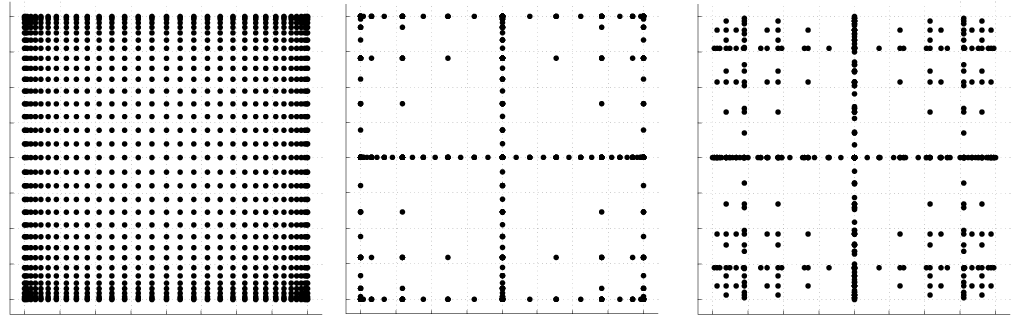
\includegraphics[width=6.5in]{images/isogrid_N2_q6}
\caption{Two-dimensional grid comparison with a tensor product grid
  using Clenshaw-Curtis points (left) and sparse grids
  $\mathscr{A}(5,2)$ utilizing Clenshaw-Curtis (middle) and
  Gauss-Legendre (right) points with nonlinear growth. }
\label{fig:isogrid_N2_q7}
\end{center}
\end{figure}

%Figure~\ref{fig:pascal_sparse_lev4_Gauss} depicts the monomial
%coverage in Pascal's triangle for two-dimensional level 4 isotropic
%sparse grids ($\mathscr{A}(4,2)$) employing the same one-dimensional
%Gaussian integration rule, where
%Figure~\ref{fig:pascal_sparse_lev4_Gauss}(a) shows the application of
%a nonlinear growth rule as given in Eq.~\ref{eq:growth_Gauss_nonlin}
%and Figure~\ref{fig:pascal_sparse_lev4_Gauss}(b) shows the use of a
%linear growth rule as given in Eq.~\ref{eq:growth_Gauss_lin}.  Using
%this geometric interpretation, subtracted tensor-product grids from
%Eqs.~\ref{eq:delta} and \ref{eq:smolyak2} can be interpreted as
%regions of overlap where only a single contribution to the integral
%should be retained.  And for these monomial coverage patterns, the
%traditional approach of exploying a total-order PCE (maximal
%resolvable total-order integrand depicted with red horizontal line)
%can be seen to be well synchronized for the case of linear growth
%rules (since only a few small ``teeth'' protrude beyond the maximal
%total-order basis) and to be somewhat conservative for nonlinear
%growth rules due to the ``hyperbolic cross'' shape (since the maximal
%total-order basis is dictated by the concave interior, neglecting the
%extended coverage along the axes).
%
%However, the inclusion of additional terms beyond the
%total-order basis in the nonlinear growth rule case, as motivated by
%the legs in Figure~\ref{fig:pascal_sparse_lev4_Gauss}(a), would be
%error-prone, since the order of the unknown response function will
%tend to push the product integrand (Eq.~\ref{eq:coeff_extract}) out
%into the concave interior, resulting in product polynomials that are
%not resolvable by the sparse integration.
%\begin{figure}[htbp]
%  \begin{subfigmatrix}{2}
%  \subfigure[Nonlinear growth rule.]{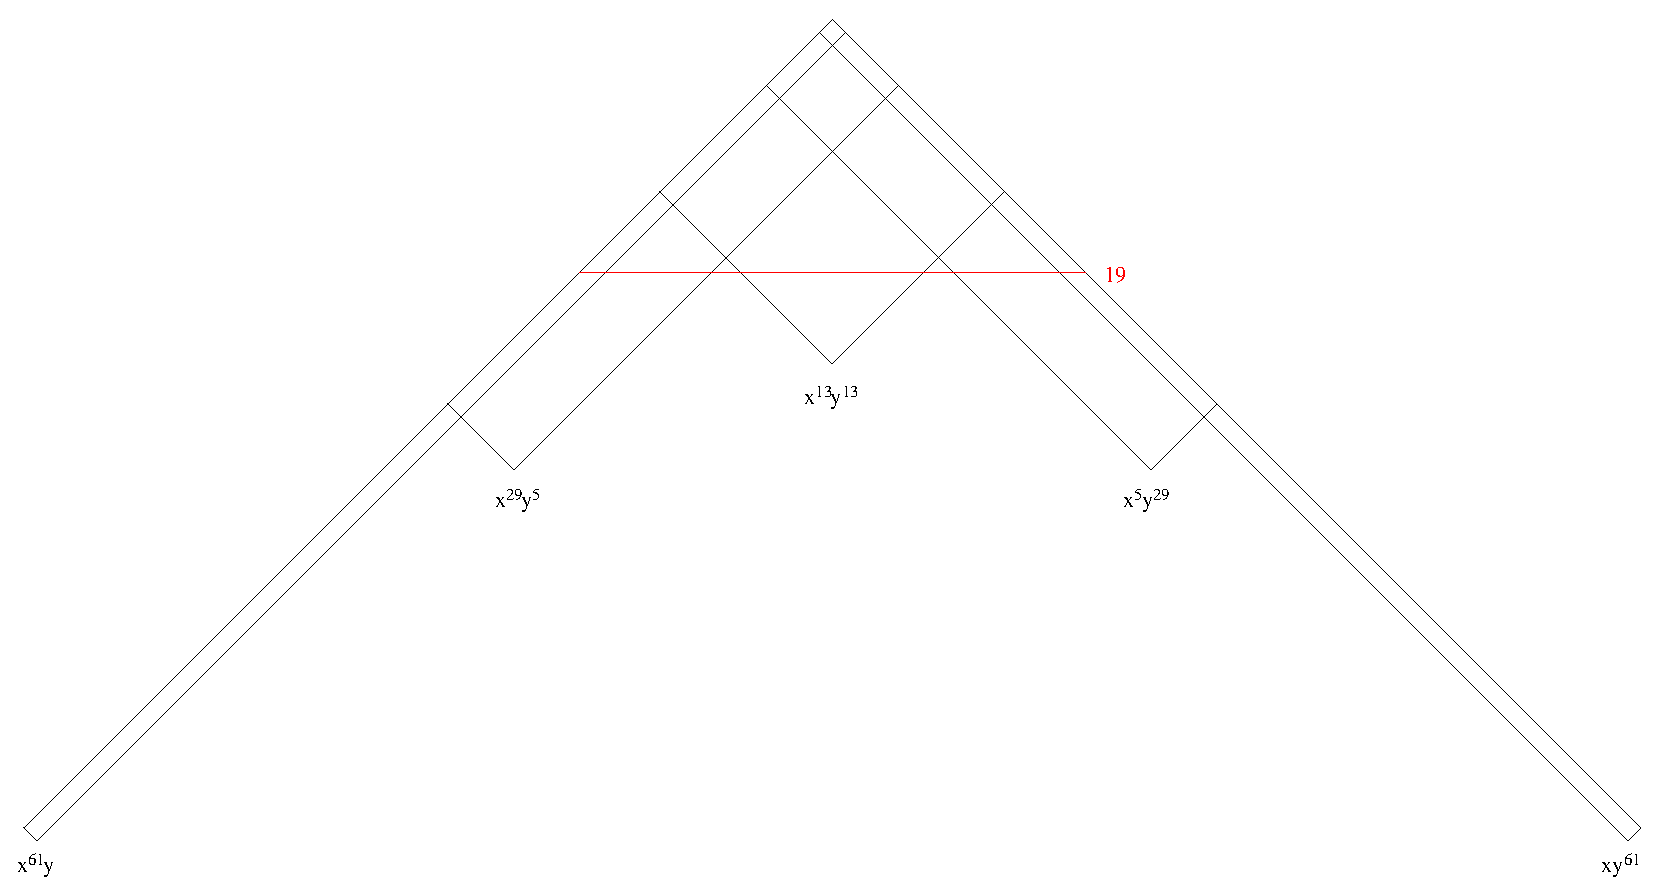
\includegraphics{SparseLevel4_NonlinGauss}}
%  \subfigure[Linear growth rule.]{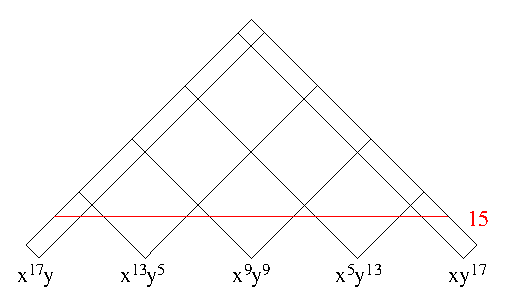
\includegraphics{SparseLevel4_LinGauss}}
%  \end{subfigmatrix}
%  \caption{Pascal's triangle depiction of integrand monomial coverage 
%for two dimensions and Gaussian sparse grid level = 4.  Red line depicts 
%maximal total-order integrand coverage.}
%\label{fig:pascal_sparse_lev4_Gauss}
%\end{figure}
%For the total-order PCE basis, the integrand monomial coverage must
%again resolve $2p$, such that $p = 9$ would be selected in this
%nonlinear growth rule example and $p = 7$ would be selected in the
%linear growth rule example.

In~\cite{Eld09a}, it is demonstrated that the synchronization of
total-order PCE with the monomial resolution of a sparse grid is
imperfect, and that sparse grid SC consistently outperforms sparse
grid PCE when employing the sparse grid to directly evaluate the
integrals in Eq.~\ref{eq:coeff_extract}.  In our DAKOTA implementation, we 
depart from the use of sparse integration of total-order expansions, and 
instead employ a linear combination of tensor expansions~\cite{ConstSSG}.
%That is, instead of employing the sparse grid as a separate numerical
%integration scheme for evaluations of Eq.~\ref{eq:coeff_extract} (for 
%which expansion synchronization is a challenge), we instead 
That is, we compute separate tensor polynomial chaos expansions for
each of the underlying tensor quadrature grids (for which there is no
synchronization issue) and then sum them using the Smolyak
combinatorial coefficient (from Eq.~\ref{eq:smolyak2} in the isotropic
case).  This improves accuracy, preserves the PCE/SC consistency
property described in Section~\ref{uq:expansion:spectral_quad}, and also
simplifies PCE for the case of anisotropic sparse grids described next.

For anisotropic Smolyak sparse grids, a dimension preference vector is
used to emphasize important stochastic dimensions.  
%A natural mechanism for quantifying
%dimension importance is through the global sensitivity analysis
%procedure described in Section~\ref{sec:ssa:global}, as the
%attribution of output variance among input sources provides an
%intuitive measure of importance in the stochastic setting.
Given a mechanism for defining anisotropy, we can extend the
definition of the sparse grid from that of Eq.~\ref{eq:smolyak2} to
weight the contributions of different index set components.  First,
the sparse grid index set constraint becomes
\begin{equation}
{\rm w}\underline{\gamma} < \mathbf{i} \cdot \mathbf{\gamma} \leq 
{\rm w}\underline{\gamma}+|\mathbf{\gamma}|
\label{eq:aniso_smolyak_constr}
\end{equation}
where $\underline{\gamma}$ is the minimum of the dimension weights
$\gamma_k$, $k$ = 1 to $n$.  The dimension weighting vector
$\mathbf{\gamma}$ amplifies the contribution of a particular dimension
index within the constraint, and is therefore inversely related to the
dimension preference (higher weighting produces lower index set
levels).  For the isotropic case of all $\gamma_k = 1$, it is evident
that you reproduce the isotropic index constraint ${\rm w}+1 \leq
|\mathbf{i}| \leq {\rm w}+n$ (note the change from $<$ to $\leq$).
Second, the combinatorial coefficient for adding the contribution from
each of these index sets is modified as described in~\cite{Burk09}.
%Given the modified index sets and combinatorial coefficients defined
%from the dimension preference vector, interpolation (SC) on
%anisotropic sparse grids proceeds as for the isotropic case.  PCE,
%however, again has the challenge of expansion tailoring.  Fortunately,
%in the anistropic case, we can assume that more is known about the
%form of the response function (especially if the dimension preference
%was based on variance-based decomposition).  This allows us to abandon
%the safe total-order basis approach in favor of a tightly-synchronized
%expansion formulation that applies the $2p$ logic to all of the
%protruding ``legs'' in the monomial resolution structure.


\subsubsection{Cubature} \label{uq:expansion:cubature}

Cubature rules~\cite{stroud,xiu_cubature} are specifically optimized
for multidimensional integration and are distinct from tensor-products 
and sparse grids in that they are not based on combinations of 
one-dimensional Gauss quadrature rules.  They have the advantage of 
improved scalability to large numbers of random variables, but are 
restricted in integrand order and require homogeneous random variable 
sets (achieved via transformation).  For example, optimal rules for
integrands of 2, 3, and 5 and either Gaussian or uniform densities 
allow low-order polynomial chaos expansions ($p=1$ or $2$) that are 
useful for global sensitivity analysis including main effects and, 
for $p=2$, all two-way interactions.


\subsection{Linear regression} \label{uq:expansion:regress}

The linear regression approach uses a
single linear least squares solution of the form:
\begin{equation}
\boldsymbol{\Psi} \boldsymbol{\alpha} = \boldsymbol{R} \label{eq:regression}
\end{equation}
to solve for the complete set of PCE coefficients
$\boldsymbol{\alpha}$ that best match a set of response values
$\boldsymbol{R}$.  The set of response values is obtained either by
performing a design of computer experiments within the density
function of $\boldsymbol{\xi}$ (point
collocation~\cite{pt_colloc1,pt_colloc2}) or from a subset of tensor
quadrature points with highest product weight (probabilistic
collocation~\cite{Tat95}).  In either case, each row of the matrix
$\boldsymbol{\Psi}$ contains the $N_t$ multivariate polynomial terms
$\Psi_j$ evaluated at a particular $\boldsymbol{\xi}$ sample.  An
over-sampling is recommended in the case of random samples
(\cite{pt_colloc2} recommends $2N_t$ samples), resulting in a least
squares solution for the over-determined system.  As for
sampling-based coefficient estimation, this approach is only valid for
PCE and does not require synchronization with monomial coverage; thus
it is common to combine this coefficient estimation approach with a
traditional total-order chaos expansion in order to keep sampling
requirements low.  In this case, simulation requirements for this
approach scale as $\frac{r(n+p)!}{n!p!}$ ($r$ is an over-sampling
factor with typical values $1 \leq r \leq 2$), which can be
significantly more affordable than isotropic tensor-product quadrature
(scales as $(p+1)^n$ for standard Gauss rules) for larger problems.
%A closely related technique is known as the ``probabilistic
%collocation'' approach.  Rather than employing random over-sampling,
%this technique uses a selected subset of $N_t$ Gaussian quadrature
%points (those with highest tensor-product weighting), which provides
%more optimal collocation locations and preserves interpolation
%properties.
Finally, additional regression equations can be obtained through the
use of derivative information (gradients and Hessians) from each
collocation point, which can aid in scaling with respect to the number
of random variables, particularly for adjoint-based derivative
approaches.


\subsection{Analytic moments} \label{uq:expansion:moment}

Mean and covariance of polynomial chaos expansions are available
in simple closed form:
\begin{eqnarray}
\mu_i      &=& \langle R_i \rangle ~~\cong~~ \sum_{k=0}^P \alpha_{ik} \langle 
\Psi_k(\boldsymbol{\xi}) \rangle ~=~ \alpha_{i0} \label{eq:mean_pce} \\
\Sigma_{ij} &=& \langle (R_i - \mu_i)(R_j - \mu_j) \rangle ~~\cong~~ 
%\langle (\sum_{j=1}^P \alpha_j \Psi_j(\boldsymbol{\xi}))^2 \rangle ~=~ 
\sum_{k=1}^P \sum_{l=1}^P \alpha_{ik} \alpha_{jl}
\langle \Psi_k(\boldsymbol{\xi}) \Psi_l(\boldsymbol{\xi}) \rangle ~=~
\sum_{k=1}^P \alpha_{ik}\alpha_{jk} \langle \Psi^2_k \rangle~~~~~~~~ \label{eq:covar_pce} 
\end{eqnarray}
where the norm squared of each multivariate polynomial is computed
from Eq.~\ref{eq:norm_squared}.  These expressions provide exact moments 
of the expansions, which converge under refinement to moments of the 
true response functions.
%Higher moments are also available
%analytically and could be employed in moment fitting approaches (i.e.,
%Pearson and Johnson models) in order to approximate a response PDF,
%although this is outside the scope of the current paper.

Similar expressions can be derived for stochastic collocation:
\begin{eqnarray}
\mu_i      &=& \langle R_i \rangle ~~\cong~~ \sum_{k=1}^{N_p} r_{ik} \langle 
\boldsymbol{L}_k(\boldsymbol{\xi}) \rangle ~=~ \sum_{k=1}^{N_p} r_{ik} w_k 
\label{eq:mean_sc} \\
\Sigma_{ij} &=& \langle R_i R_j \rangle - \mu_i \mu_j
~~\cong~~ \sum_{k=1}^{N_p} \sum_{l=1}^{N_p} r_{ik} r_{jl} \langle
\boldsymbol{L}_k(\boldsymbol{\xi}) \boldsymbol{L}_l(\boldsymbol{\xi}) \rangle
- \mu_i \mu_j ~=~ \sum_{k=1}^{N_p} r_{ik} r_{jk} w_k - \mu_i \mu_j~~~~~~~~~ \label{eq:covar_sc} 
\end{eqnarray}
where we have simplified the expectation of Lagrange polynomials
constructed at Gauss points and then integrated at these same Gauss
points.  For tensor grids and sparse grids with fully nested rules,
these expectations leave only the weight corresponding to the point
for which the interpolation value is one, such that the final
equalities in Eqs.~\ref{eq:mean_sc}--\ref{eq:covar_sc} hold precisely.
For sparse grids with non-nested rules, however, interpolation error
exists at the collocation points, such that these final equalities
hold only approximately.  In this case, we have the choice of
computing the moments based on sparse numerical integration or based
on the moments of the (imperfect) sparse interpolant, where small
differences may exist prior to numerical convergence.  In DAKOTA, we
employ the former approach; i.e., the right-most expressions in
Eqs.~\ref{eq:mean_sc}--\ref{eq:covar_sc} are employed for all tensor
and sparse cases irregardless of nesting.  Skewness and kurtosis
calculations as well as sensitivity derivations in the following
sections are also based on this choice.
%Similarly, moment $k$ for stochastic collocation is just 
%$\sum_{j=1}^{N_p} r^k_j w_j$ minus previously computed moments.
The expressions for skewness and (excess) kurtosis from direct numerical 
integration of the response function are as follows:
\begin{eqnarray}
\gamma_{1_i} &=& \left\langle \left(\frac{R_i - \mu_i}{\sigma_i}\right)^3 \right\rangle
~~\cong~~ \frac{1}{\sigma_i^3} \left[ \sum_{k=1}^{N_p} (r_{ik}-\mu_i)^3 w_k \right] \label{eq:skewness} \\
\gamma_{2_i} &=& \left\langle \left(\frac{R_i - \mu_i}{\sigma_i}\right)^4 \right\rangle - 3 
~~\cong~~ \frac{1}{\sigma_i^4} \left[ \sum_{k=1}^{N_p} (r_{ik}-\mu_i)^4 w_k \right] - 3\label{eq:kurtosis} 
\end{eqnarray}


\subsection{Local sensitivity analysis: derivatives with respect to expansion variables} \label{uq:expansion:rvsa}

Polynomial chaos expansions are easily differentiated with respect to
the random variables~\cite{reagan_sens}.  First, using
Eq.~\ref{eq:pc_exp_trunc},
\begin{equation}
\frac{dR}{d\xi_i} = \sum_{j=0}^P \alpha_j 
\frac{d\Psi_j(\boldsymbol{\xi})}{d\xi_i}\label{eq:dR_dxi_pce}
\end{equation}
and then using Eq.~\ref{eq:multivar_prod}, 
\begin{equation}
\frac{d\Psi_j(\boldsymbol{\xi})}{d\xi_i} = \frac{d\psi_i}{d\xi_i}
\prod_{\stackrel{\scriptstyle k=1}{k \ne i}}^n \psi_{m_k^j}(\xi_k)
\label{eq:deriv_prod_pce}
\end{equation}
where the univariate polynomial derivatives $\frac{d\psi_i}{d\xi_i}$
have simple closed form expressions for each polynomial in the Askey
scheme~\cite{abram_stegun}.  Finally, using the Jacobian of the
(extended) Nataf variable transformation,
\begin{equation}
\frac{dR}{dx_i} = \frac{dR}{d\boldsymbol{\xi}} 
\frac{d\boldsymbol{\xi}}{dx_i} \label{eq:dR_dx}
\end{equation}
which simplifies to $\frac{dR}{d\xi_i} \frac{d\xi_i}{dx_i}$ in the
case of uncorrelated $x_i$.  

Similar expressions may be derived for stochastic collocation, starting
from Eq.~\ref{eq:sc_exp_short}:
\begin{equation}
\frac{dR}{d\xi_i} = \sum_{j=1}^{N_p} r_j 
\frac{d\boldsymbol{L}_j(\boldsymbol{\xi})}{d\xi_i}\label{eq:dR_dxi_sc}
\end{equation}
where the multidimensional interpolant $\boldsymbol{L}_j$ is formed
over either tensor-product quadrature points or a Smolyak sparse grid.
For the former case, the derivative of the multidimensional
interpolant $\boldsymbol{L}_j$ involves a product rule of the
one-dimensional interpolants $L_k$:
\begin{equation}
\frac{d\boldsymbol{L}_j(\boldsymbol{\xi})}{d\xi_i} = \frac{dL_i}{d\xi_i}
\prod_{\stackrel{\scriptstyle k=1}{k \ne i}}^n L_k(\xi_k)
\label{eq:deriv_prod_sc}
\end{equation}
and for the latter case, the derivative involves a linear combination
of these product rules, as dictated by the Smolyak recursion shown in
Eq.~\ref{eq:smolyak2}.  Finally, calculation of $\frac{dR}{dx_i}$
involves the same Jacobian application shown in Eq.~\ref{eq:dR_dx}.

\subsection{Global sensitivity analysis: variance-based decomposition}\label{uq:expansion:vbd}

In addition to obtaining derivatives of stochastic expansions with 
respect to the random variables, it is possible to obtain 
variance-based sensitivity indices from the stochastic expansions. 
Variance-based sensitivity indices are explained in 
Section~\ref{dace:sensitivity}.  The concepts are summarized here 
as well.  Variance-based decomposition 
is a global sensitivity method that summarizes how the uncertainty 
in model output can be apportioned to uncertainty in individual 
input variables.  VBD uses two primary measures, the main effect 
sensitivity index $S_{i}$ and the total effect index $T_{i}$.  These 
indices are also called the Sobol' indices. The main effect sensitivity 
index corresponds to the fraction of the uncertainty in the output, $Y$, 
that can be attributed to input $x_{i}$ alone.  The total effects index 
corresponds to the fraction of the uncertainty in 
the output, $Y$, that can be attributed to input $x_{i}$ and its 
interactions with other variables. The main effect sensitivity index
compares the variance of the conditional expectation
$Var_{x_{i}}[E(Y|x_{i})]$ against the total variance $Var(Y)$.
Formulas for the indices are: 

\begin{equation}
S_{i}=\frac{Var_{x_{i}}[E(Y|x_{i})]}{Var(Y)} \label{eq:sobol}
\end{equation}

and 
\begin{equation}
T_{i}=\frac{E(Var(Y|x_{-i}))}{Var(Y)}=\frac{Var(Y)-Var(E[Y|x_{-i}])}{Var(Y)}
\label{eq:total_sobol}
\end{equation}

where $Y=f({\bf x})$ and ${x_{-i}=(x_{1},...,x_{i-1},x_{i+1},...,x_{m})}$.

The calculation of $S_{i}$ and $T_{i}$ requires the evaluation of 
m-dimensional integrals which are typically approximated by Monte-Carlo 
sampling. However, in stochastic expansion methods, it is possible to 
obtain the sensitivity indices as analytic functions of the 
coefficients in the stochastic expansion.  The derivation 
of these results is presented in ~\cite{Tang10b}. The sensitivity 
indices are printed as a default when running either 
polynomial chaos or stochastic collocation in DAKOTA. 
Note that in addition to the first-order main effects, $S_{i}$, 
we are able to calculate the sensitivity indices for higher order 
interactions such as the two-way interaction  $S_{i,j}$.   

\subsection{Automated Refinement}\label{uq:expansion:refine}

Several approaches for refinement of stochastic expansions are
presented here: uniform p-refinement with isotropic sparse and tensor
grids, adaptive p-refinement using anisotropic sparse and tensor
grids, and goal-oriented adaptive p-refinement using generalized
sparse grids.  Each involves incrementing the grid upon which the 
stochastic expansions are based, using differing refinement criteria
and convergence controls.

\subsubsection{Uniform p-refinement with isotropic grids}

Uniform p-refinement involves ramping the order of a tensor-product
quadrature grid or the level of a Smolyak sparse grid isotropically.
In this case, dimension preferences are not computed, and the only
algorithmic requirements are:
\begin{itemize}
\item With the usage of nested integration rules with restricted
  exponential growth, DAKOTA must ensure that a change in level
  results in a sufficient change in the grid; otherwise premature
  convergence could occur within the refinement process.  If no change
  is initially detected, DAKOTA continues incrementing the order/level
  (without grid evaluation) until the number of grid points increases.
\item A convergence criterion is required.  For uniform refinement,
  DAKOTA employs the $L^2$ norm of the change in the response
  covariance matrix as a general-purpose convergence metric.
\end{itemize}


\subsubsection{Adaptive p-refinement with anisotropic grids}

Adaptive p-refinement involves ramping the order of a tensor-product
quadrature grid or the level of a Smolyak sparse grid anisotropically,
that is, using a defined dimension preference.  This dimension
preference may be computed from local sensitivity analysis, global
sensitivity analysis, a posteriori error estimation, or decay rate
estimation.  In the current release, we focus on global sensitivity
analysis from low order isotropic expansions where dimension
preference is defined from total Sobol' indices
(Eq.~\ref{eq:total_sobol}) and is updated on every iteration.  This
dimension preference vector supports anisotropic sparse grids based on
a linear index-set constraint (Eq.~\ref{eq:aniso_smolyak_constr}) or
anisotropic tensor grids (Eq.~\ref{eq:multi_tensor}) with dimension
order scaled proportionately to preference; in both cases, dimension
refinement lower bound constraints are enforced to ensure that all
previously evaluated points remain in new refined grids.
%; with the introduction of interaction effects, nonlinear index-set
%constraints can also be considered.


\subsubsection{Goal-oriented p-refinement with generalized sparse grids}

The uniform and adaptive refinement capabilities described above
define anisotropy and control convergence in a highly structured
manner based on variance-related measures.  The generalized sparse
grid algorithm~\cite{Gerstner_Griebel_2003}, on the other hand,
supports greater flexibility in the definition of sparse grid index
sets and supports refinement controls based on general statistical
quantities of interest (QOI).  This algorithm was originally intended
for adaptive numerical integration on a hypercube, but can be readily
extended to the adaptive refinement of stochastic expansions using 
the following customizations:
\begin{itemize}
\item In addition to hierarchical interpolants in SC, we employ
  independent polynomial chaos expansions for each active and accepted
  index set.  Pushing and popping index sets then involves increments
  of tensor chaos expansions (as described in
  Section~\ref{uq:expansion:spectral_sparse}) along with corresponding
  increments to the Smolyak combinatorial coefficients.
\item Since we support bases for more than uniform distributions on a
  hypercube, we exploit rule nesting when possible (i.e.,
  Gauss-Patterson for uniform or transformed uniform variables, and
  Genz-Keister for normal or transformed normal variables), but we do
  not require it.  This implies a loss of some algorithmic
  simplifications in~\cite{Gerstner_Griebel_2003} that occur when
  grids are strictly hierarchical.
\item In the evaluation of the effect of a trial index set, the goal
  in~\cite{Gerstner_Griebel_2003} is numerical integration and the
  metric is the size of the increment induced by the trial set on the
  expectation of the function of interest.  It is straightforward to
  instead measure the effect of a trial index set on response
  covariance, numerical probability, or other statistical QOI
  computed by post-processing the resulting PCE or SC expansion.  
  %(it is much less straightforward to embed QOI in the calculation
  %of dimension preference for anisotropic tensor/sparse grids).
  By tying the refinement process more closely to the statistical QOI,
  the refinement process can become more efficient in achieving the
  desired analysis objectives.
\end{itemize}

%If the objectives and constraints of a design under uncertainty
%problem are focused on variance (e.g., robust design), then the
%general-purpose formulations described above are sufficiently
%goal-oriented.  However, for other classes of problems (e.g.,
%reliability-based design or stochastic inverse problems), we may
%prefer to employ refinement approaches guided by assessments of
%accuracy in other statistical quantities of interest.  A particular
%focus in this effort is to refine adaptively with the goal of
%accuracy in tail probability estimates.  There are two parts to this
%effort: goal-oriented p-refinement using generalized sparse grids
%and efficient tail probability estimation.
%
%Since probability levels are not available analytically from
%stochastic expansions, they must be evaluated numerically using some
%form of sampling on the expansion.  For tail probability estimates,
%standard sampling approaches (e.g., LHS) can become expensive even for
%this surrogate-based sampling and we require a more directed
%probability estimation procedure, in particular the importance
%sampling procedure described previously in Section~\ref{sec:imp_samp}.

Given these customizations, the algorithmic steps can be summarized as:
\begin{enumerate}
\item {\em Initialization:} Starting from an initial isotropic or
  anisotropic reference grid (often the $w=0$ grid corresponding to a
  single collocation point), accept the reference index sets as the
  old set and define active index sets using the admissible forward
  neighbors of all old index sets.
\item {\em Trial set evaluation:} Evaluate the tensor grid
  corresponding to each trial active index set, form the tensor
  polynomial chaos expansion or tensor interpolant corresponding to
  it, update the Smolyak combinatorial coefficients, and combine the
  trial expansion with the reference expansion.  Perform necessary
  bookkeeping to allow efficient restoration of previously evaluated
  tensor expansions.
\item {\em Trial set selection:} Select the trial index set that
  induces the largest change in the statistical quantity of interest.
  In our implementation, we employ an $L^2$ norm of change in CDF/CCDF
  probability/reliability/response level mappings, when level mappings
  are present, or $L^2$ norm of change in response covariance, when
  level mappings are not present.
\item {\em Update sets:} If the largest change induced by the trial
  sets exceeds a specified convergence tolerance, then promote the
  selected trial set from the active set to the old set and update the
  active sets with new admissible forward neighbors; return to step 2
  and evaluate all trial sets with respect to the new reference point.
  If the convergence tolerance is satisfied, advance to step 5.
\item {\em Finalization:} Promote all remaining active sets to the old
  set, update the Smolyak combinatorial coefficients, and perform a
  final combination of tensor expansions to arrive at the final result
  for the statistical quantity of interest.
\end{enumerate}


\subsection{Uncertainty Quantification Example using Stochastic Collocation}\label{uq:uncertainty2}

A typical DAKOTA input file for performing an uncertainty
quantification using polynomial chaos expansions is shown in the
Tutorial Chapter,
Section~\ref{tutorial:example:uncert_quant:poly_chaos}.  The example
in the Tutorial Chapter illustrates PCE built on anisotropic tensor
product quadrature.  The uncertain variables are uniforms, so the
expansion is built using classical Legendre polynomials. This section
presents a more sophisticated example, where we use stochastic
collocation built on an anisotropic sparse grid defined from
numerically-generated orthogonal polynomials.  The uncertain variables
are lognormal in this example and the orthogonal polynomials are
generated from Gauss-Wigert recursion coefficients~\cite{simpson_gw}
in combination with the Golub-Welsch procedure~\cite{GolubWelsch69}.
The input file is shown in Figure~\ref{uq:figure11}. This 
input file is \texttt{dakota\_sc.in} in the 
\texttt{Dakota/examples/methods} directory.  Note that the
dimension preference of $(2,1)$ is inverted to define a $\gamma$
weighting vector of $(0.5,1)$ (and $\underline{\gamma}$ of $0.5$) for
use in Eq.~\ref{eq:aniso_smolyak_constr}.  In this example, we compute
CDF probabilities for six response levels of Rosenbrock's function.
This example requires 19 function evaluations to calculate the
interpolating polynomials in stochastic collocation and the resulting
expansion exactly reproduces Rosenbrock's function.  The placement of
the points generated by the sparse grid is shown in
Figure~\ref{uq:figure11b}.

\begin{figure}
  \centering
  \begin{bigbox}
    \begin{small}
      \verbatimtabinput[8]{dakota_sc.in}
    \end{small}
  \end{bigbox}
\caption{DAKOTA input file for performing UQ using stochastic collocation.}
\label{uq:figure11}
\end{figure}

\begin{figure}[ht!]
  \centering
  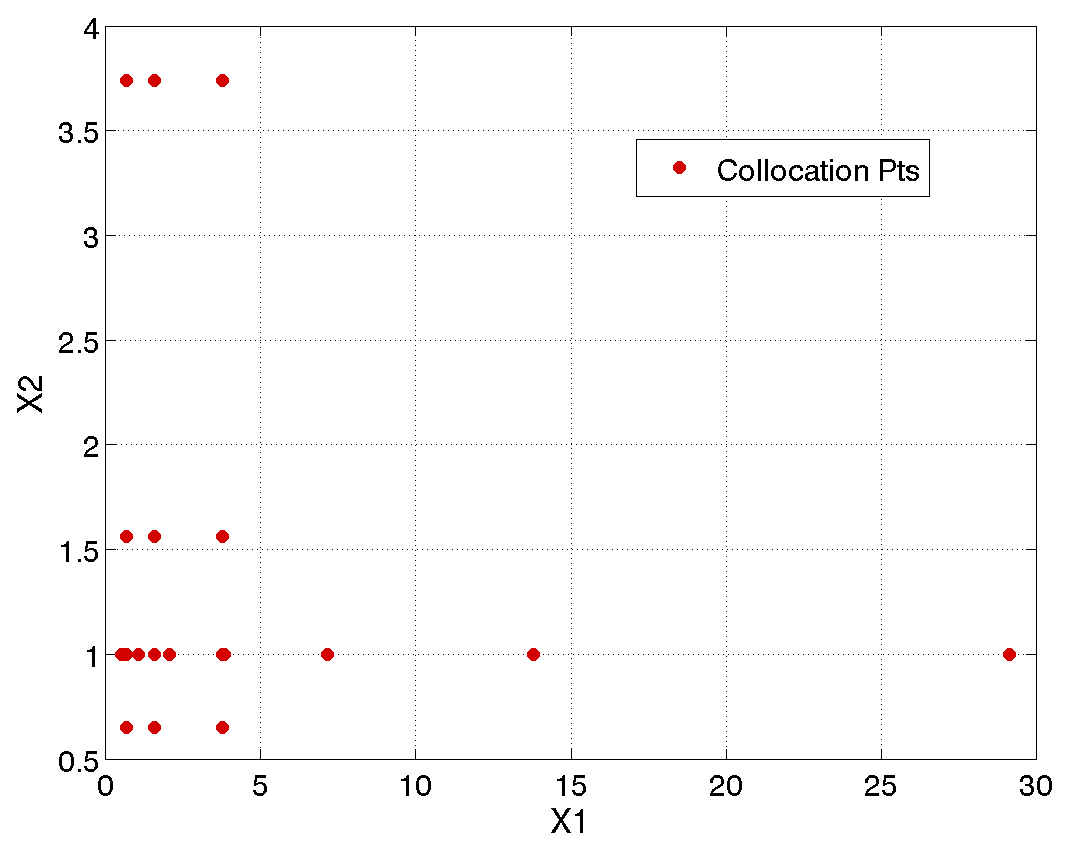
\includegraphics[height=2.5in]{images/rosen_sc_pts}
  \caption{Rosenbrock stochastic collocation example: sparse grid points.}
  \label{uq:figure11b}
\end{figure}

Once the expansion coefficients have been calculated, some statistics
are available analytically and others must be evaluated numerically.
For the numerical portion, the input file specifies the use of 10000
samples, which will be evaluated on the expansion to compute the CDF
probabilities.  In Figure~\ref{uq:figure12}, excerpts from the results
summary are presented.  We first see the analytic statistics for 
mean and standard deviation as computed from 
Eqs.~\ref{eq:mean_sc}-\ref{eq:covar_sc} as well as skewness, and kurtosis.  
The response covariance (collapsing to a single variance value for 
one response function) and global sensitivity indices
(Sobol' indices) are presented next. This example shows that variable 
x1 has the largest main effect (0.99) as compared with variable 
x2 (0.0007) or the interaction between x1 and x2 (0.005). 
%After the global sensitivity indices, the local, analytic random 
%variable sensitivities are presented, as computed from
%Eqs.~\ref{eq:dR_dx}-\ref{eq:dR_dxi_sc}, evaluated at the mean values.
Finally, we see the numerical results for the CDF probabilities based
on 10000 samples performed on the expansion.  For example, the probability 
that the Rosenbrock function is less than 100 is 0.7233.  Note that these 
results are significantly different than the ones presented in 
Section~\ref{tutorial:example:uncert_quant:poly_chaos} because of 
the different assumptions about the inputs: uniform[-2,2] versus
lognormals with means of 1.0 and standard deviations of 0.5. 
\begin{figure}
\centering
\begin{bigbox}
\begin{footnotesize}
\begin{verbatim}
Statistics derived analytically from polynomial expansion:

Moment-based statistics for each response function:
                            Mean           Std Dev          Skewness          Kurtosis
 response_fn_1  2.5671972656e+02  2.0484189184e+03  2.7419241630e+02  1.9594567379e+06

Covariance among response functions:
[[  4.1960200651e+06 ]] 

Global sensitivity indices for each response function:
response_fn_1 Sobol indices:
                                  Main             Total
                      9.9391978710e-01  9.9928724777e-01 x1
                      7.1275222945e-04  6.0802128961e-03 x2
                           Interaction
                      5.3674606667e-03 x1 x2 

Statistics based on 10000 samples performed on polynomial expansion:

Level mappings for each response function:
Cumulative Distribution Function (CDF) for response_fn_1:
     Response Level  Probability Level  Reliability Index  General Rel Index
     --------------  -----------------  -----------------  -----------------
   1.0000000000e-01   1.8100000000e-02
   1.0000000000e+00   8.7800000000e-02
   5.0000000000e+01   5.8410000000e-01
   1.0000000000e+02   7.2330000000e-01
   5.0000000000e+02   9.2010000000e-01
   1.0000000000e+03   9.5660000000e-01
\end{verbatim}
\end{footnotesize}
\end{bigbox}
\caption{Excerpt of UQ output for stochastic collocation example.}
\label{uq:figure12}
\end{figure}

\section{Epistemic Nondeterministic Methods}\label{uq:epistemic}

Uncertainty quantification is often used as part of the risk
assessment of performance, reliability, and safety of engineered
systems.  Increasingly, uncertainty is separated into two categories
for analysis purposes: aleatory and epistemic
uncertainty~\cite{Obe03,Hel07}. Aleatory uncertainty is also referred to as
variability, irreducible or inherent uncertainty, or uncertainty due
to chance. Examples of aleatory uncertainty include the height of
individuals in a population, or the temperature in a processing
environment.  Aleatory uncertainty is usually modeled with probability
distributions, and sampling methods such as Latin Hypercube sampling
in DAKOTA can be used to model aleatory uncertainty. In contrast,
epistemic uncertainty refers to lack of knowledge or lack of
information about a particular aspect of the simulation model,
including the system and environment being modeled. An increase in
knowledge or information relating to epistemic uncertainty will lead
to a reduction in the predicted uncertainty of the system response or
performance. For epistemic uncertain variables, typically one does not
know enough to specify a probability distribution on a variable.
Epistemic uncertainty is referred to as subjective, reducible, or lack
of knowledge uncertainty. Examples of epistemic uncertainty include
little or no experimental data for a fixed but unknown physical
parameter, incomplete understanding of complex physical phenomena,
uncertainty about the correct model form to use, etc.

There are many approaches which have been developed to model epistemic
uncertainty, including fuzzy set theory, possibility theory, and
evidence theory. It is also possible to use simple interval analysis in 
an epistemic context.  Interval analysis and evidence theory are 
described in more detail below.

\subsection{Interval Methods for Epistemic Analysis}\label{uq:interval}
In interval analysis, one assumes that nothing is known about 
an epistemic uncertain variable except that its value lies 
somewhere within an interval.  In this situation, it is NOT 
assumed that the value has a uniform probability of occuring 
within the interval.  Instead, the interpretation is that 
any value within the interval is a possible value or a potential 
realization of that variable.  In interval analysis, the 
uncertainty quantification problem is one of determining the 
resulting bounds on the output (defining the output interval) 
given interval bounds on the inputs. Again, any output response 
that falls within the output interval is a possible output 
with no frequency information assigned to it.

We have the capability to perform interval analysis using either
\texttt{global\_interval\_est} or \texttt{local\_interval\_est}.
In the global approach, one uses either a global optimization 
method or a sampling method to assess the bounds. 
\texttt{global\_interval\_est}
allows the user to specify either \texttt{lhs}, which performs 
Latin Hypercube Sampling and takes the minimum and maximum of 
the samples as the bounds (no optimization is 
performed) or \texttt{ego}.  In the case of \texttt{ego}, 
the efficient global optimization method is used to calculate 
bounds.  The ego method is described in Section~\ref{sbm:egm}.
If the problem is amenable to local optimization 
methods (e.g. can provide derivatives or use finite difference 
method to calculate derivatives), then one can use local
methods to calculate these bounds.  \texttt{local\_interval\_est}
allows the user to specify either \texttt{sqp} which is sequential 
quadratic programming, or \texttt{nip} which is a nonlinear interior point 
method. 

Note that when performing interval analysis, it is necessary to 
define interval uncertain variables as described in 
Section~\ref{variables:uncertain}.  For interval analysis, 
one must define only one interval per input variable, in 
contrast with Dempster-Shafer evidence theory, where 
an input can have several possible intervals.  Interval 
analysis can be considered a subset of Dempster-Shafer
evidence theory where each input is defined by one 
input interval with a basic probability assignment of one. 
If you are performing a pure interval analysis, we 
recommend using either \texttt{global\_interval\_est} or 
\texttt{local\_interval\_est}.  An example of interval estimation 
is found in the test file \texttt{dakota\_uq\_cantilever\_interval.in}, 
and also in the Tutorial, Section~\ref{tutorial:example:uncert_quant:interval}. 
Note that we have kept separate 
implementations of interval analysis and Dempster-Shafer 
evidence theory because our users often want to couple 
interval analysis on an ``outer loop'' with an aleatory, 
probabilistic analysis on an ``inner loop'' for nested, 
second-order probability calculations.  See Section~\ref{models:ex:sop} 
for more details on nested approaches.


\subsection{Dempster-Shafer Theory of Evidence}\label{uq:dempshaf}
We have chosen to pursue evidence theory at Sandia as a way to 
model epistemic uncertainty, in part because evidence theory is
a generalization of probability theory.  Evidence theory is also
referred to as Dempster-Shafer theory or the theory of random
sets~\cite{Obe03}.  In evidence theory, there are two complementary
measures of uncertainty: belief and plausibility.  Together, belief
and plausibility can be thought of as defining lower and upper bounds,
respectively, on probabilities.  Belief and plausibility define the
lower and upper limits or intervals on probability values. 
Typical plots of cumulative and complementary cumulative 
belief and plausibility functions are shown in 
Figure~\ref{uq:figure15}~\cite{Hel07}.  
In evidence theory, it is not possible to specify one probability value.
Instead, there is a range of values that is consistent with the
evidence. The range of values is defined by belief and
plausibility. Note that no statement or claim is made about one value
within an interval being more or less likely than any other value.

This section focuses on Dempster-Shafer evidence theory.  We also 
use a technique called second-order probability to perform 
uncertainty quantification when there is both epistemic and 
aleatory uncertainty present.  Second-order probability is a nested 
technique with two levels of uncertainty quantification.  
The outer level UQ is typically linked 
to epistemic uncertainties and the inner level UQ is commonly associated 
with aleatory uncertainties.  A common approach used is to sample 
possible realizations of epistemic variables in the outer loop, 
then send these to the inner loop for additional sampling over the aleatory 
variables.  In this way one generates ``families'' or ensembles of 
cumulative distribution functions, where each individual CDF is based on 
aleatory uncertainty, and the ensemble is based on epistemic uncertainty. 
See Section~\ref{models:ex:sop} for more details.

\begin{figure}
  \centering 
  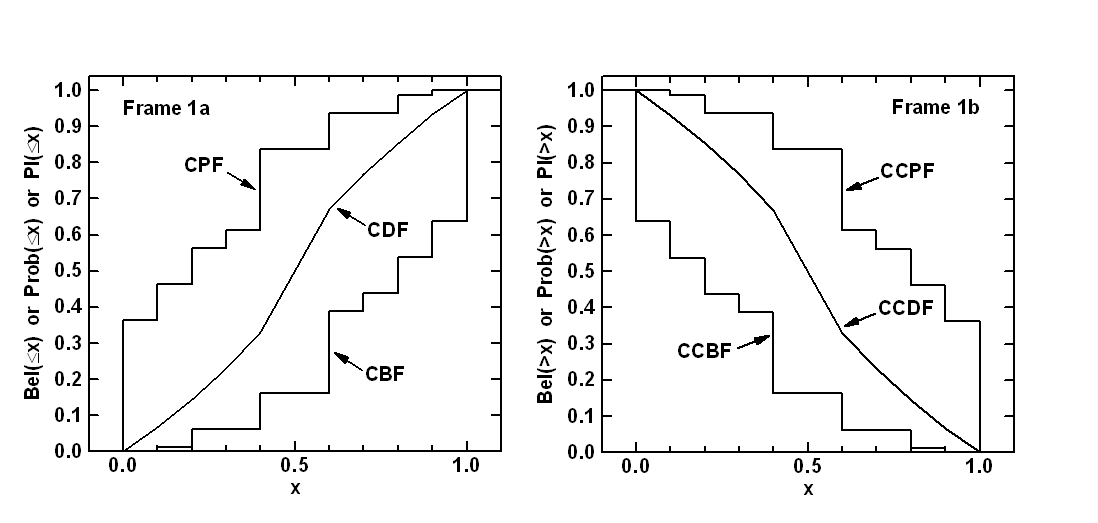
\includegraphics[scale=0.8]{images/belief_plaus} 
  \caption{Example cumulative belief and plausibility distribution functions on left; complementary cumulative belief and plausibility distribution functions on right}
  \label{uq:figure15}
\end{figure}

In Dempster-Shafer evidence theory, the uncertain input variables are
modeled as sets of intervals.  The user assigns a basic probability
assignment (BPA) to each interval, indicating how likely it is that
the uncertain input falls within the interval.  The BPAs for a
particular uncertain input variable must sum to one.  The intervals
may be overlapping, contiguous, or have gaps. In DAKOTA, an interval
uncertain variable is specified as \texttt{interval\_uncertain}.  When
one defines an interval type variable in DAKOTA, it is also necessary
to specify the number of intervals defined for each variable with
\texttt{iuv\_num\_intervals} as well the basic probability assignments
per interval, \texttt{iuv\_interval\_probs}, and the associated bounds
per each interval, \texttt{iuv\_interval\_bounds}. 
Figure~\ref{uq:figure16} shows the input specification for interval
uncertain variables. This input file is \texttt{dakota\_uq\_textbook\_dste.in}, found in the \texttt{Dakota/examples/methods} 
directory.   The example shown in Figure~\ref{uq:figure16}
has two epistemic uncertain interval variables.  
The first uncertain
variable has three intervals and the second has two. The basic
probability assignments for the first variable are 0.5, 0.1, and 0.4,
while the BPAs for the second variable are 0.7 and 0.3. Note that it
is possible (and often the case) to define an interval uncertain
variable with only ONE interval.  This means that you only know that
the possible value of that variable falls within the interval, and the
BPA for that interval would be 1.0.  In the case we have shown, the
interval bounds on the first interval for the first variable are 0.6
and 0.9, and the bounds for the second interval for the first variable
are 0.1 to 0.5, etc.

\begin{figure}
  \centering
  \begin{bigbox}
    \begin{small}
      \verbatimtabinput[8]{dakota_uq_textbook_dste.in}
    \end{small}
  \end{bigbox}
\caption{DAKOTA input file for UQ example using Evidence Theory.}
\label{uq:figure16}
\end{figure}

Once the intervals, the BPAs, and the interval bounds are defined, 
the user can run an epistemic analysis by specifying the method as 
either \texttt{global\_evidence} or 
\texttt{local\_evidence} in the DAKOTA input file.  
Both of these methods perform Dempster-Shafer calculations:  
the difference is that the local method uses a local optimization 
algorithm to calculate the interval bounds and the global 
method uses either sampling or a global optimization approach to 
calculate an interval bound.  These differences are discussed in 
more detail below. 
The intervals and their associated BPAs are then propagated through
the simulation to obtain cumulative distribution functions on belief
and plausibility.  As mentioned above, belief is the lower bound on a
probability estimate that is consistent with the evidence, and
plausibility is the upper bound on a probability estimate that is
consistent with the evidence.  

Figure~\ref{uq:figure17} shows
results for the first response function obtained when running the
example in Figure~\ref{uq:figure16}.  In this example, there are 6
output intervals (as a result of the 2 interval input variables with 3
and 2 intervals, respectively). 
The output intervals are ordered to obtain cumulative
bound functions for both belief and plausibility.  The
cumulative distribution function is presented for both belief (CBF) and
plausibility (CPF).  The CBF value is the cumulative belief
corresponding to a certain output value.  For example, the belief that
the output value is less than or equal to 0.2 for response 1 is 0.27, 
and the plausibility that the output is less than
or equal to 0.2 is 1 for response 1.  The belief that the 
output value is less than 0.6217 is 0.75, while the plausbility that 
the output is less than  0.0806 is 0.75.  
The CBF and CPF may be plotted on a graph and
interpreted as bounding the cumulative distribution
function (CDF), which is the probability that the output is less than or equal
to a certain value. The interval bounds on probability values show
the value of epistemic uncertainty analysis: the intervals are usually
much larger than expected, giving one a truer picture of the total
output uncertainty caused by lack of knowledge or information about
the epistemic input quantities.

\begin{figure}
\centering
\begin{bigbox}
\begin{small}
\begin{verbatim}
Belief and Plausibility for each response function:
Cumulative Belief/Plausibility Functions (CBF/CPF) for response_fn_1:
     Response Level  Belief Prob Level   Plaus Prob Level
     --------------  -----------------   ----------------
   1.0000000000e-03   0.0000000000e+00   0.0000000000e+00
   3.0000000000e-02   0.0000000000e+00   2.7000000000e-01
   2.0000000000e-01   2.7000000000e-01   1.0000000000e+00
   8.0000000000e-01   9.3000000000e-01   1.0000000000e+00
  Probability Level  Belief Resp Level   Plaus Resp Level
  -----------------  -----------------   ----------------
   2.5000000000e-01   2.6187288772e-01   6.2609206069e-02
   5.0000000000e-01   2.9829775860e-01   6.3736734971e-02
   7.5000000000e-01   6.2173551556e-01   8.0596931719e-02
\end{verbatim}
\end{small}
\end{bigbox}
\caption{Results of an Epistemic Uncertainty Quantification using Evidence Theory.}
\label{uq:figure17}
\end{figure}

As in other nondeterministic methods, with \texttt{local\_evidence}
or \texttt{global\_evidence},
one can specify probability levels and response levels. 
If response levels are specified, the belief and plausibility 
function values corresponding to those response levels are calculated 
(see Belief Prob Level and Plaus Prob Level in the tables shown in 
Figure~\ref{uq:figure17}).  Similarly, if probability levels are 
specified, these are first interpreted to be belief values, and the 
corresponding response levels are calculated (see Belief Resp Level); 
then they are interpreted to be plausibility values and the 
corresponding response levels are calculated (see Plaus Resp Level in 
the table in Figure~\ref{uq:figure17}).  We have recently added the 
capability to support generalized reliability mappings in 
the evidence methods.  If the user specifies a generalized 
reliability level, it will be first converted to a probability, 
then interpreted as a belief and plausibility and the corresponding 
response levels will be calculated. Likewise, if response levels 
are specified, the corresponding belief and plausibility values 
will be mapped to bounds on the generalized reliability levels. 

To elaborate on the differences between \texttt{global\_evidence}
and \texttt{local\_evidence}: both of these methods
take the Dempster-Shafer structures specified on the inputs 
and calculate a resulting Dempster-Shafer structure on the 
outputs (e.g. a cumulative belief and plausibility function). 
To calculate the belief and plausibility measures, it is 
necessary to calculate the minimum and maximum of the response function 
in each ``interval cell combination.''  For example, in a two variable 
problem, if the first variable had three intervals and associated BPAs 
assigned and the second variable had two intervals and associated 
BPAs assigned, there would be 6 interval cells in total. 
In each of these six cells, one needs to identify a minimum and 
maximum value of the response function.  This is easy to do if 
the function is monotonic in both variables, but in general 
it is not.  We offer the capability to use local optimization 
methods to calculate these bounds: \texttt{local\_evidence}
allows the user to specify either \texttt{sqp} which is sequential 
quadratic programming, or \texttt{nip} which is a nonlinear interior point 
method.  We also offer the capability to use global methods to 
assess these interval cell bounds. \texttt{global\_evidence}
allows the user to specify either \texttt{lhs}, which performs 
Latin Hypercube Sampling and takes the minimum and maximum of 
the samples within each cell as the bounds (no optimization is 
performed) or \texttt{ego}.  In the case of \texttt{ego}, 
the efficient global optimization method is used to calculate 
bounds.  The ego method is described in Section~\ref{sbm:egm}.
Note that for a situation with many uncertain variables, 
each with a fairly complicated Dempster-Shafer structure 
described by many intervals, there will be a huge number 
of interval calls, and the overall process of performing 
Dempster-Shafer analysis will be extremely expensive. 
Reference~\cite{Tang10b} provides more details about 
the implementation of the optimization methods to perform 
Dempster-Shafer calculations, as well as comparisons on test problems.

\begin{comment}
\section{Bayesian Calibration Methods}\label{uq:bayesian}
We are currently investigating Bayesian methods,specifically focusing on 
Bayesian calibration, where a ``prior distribution'' on a parameter is 
updated through a Bayesian framework involving experimental data and 
a likelihood function. The first DAKOTA implementation of a Bayesian 
calibration capability uses the GPMSA code developed at 
Los Alamos National Laboratory.

GPMSA is a code that provides the capability for Bayesian calibration:  
given a computational simulation model with unknown parameters and 
prior distributions on those parameters, along with observational data 
(e.g. from experiments),  GPMSA uses a Monte Carlo Markov Chain (MCMC) 
algorithm to produce posterior distributions on the parameters.  
When the computational simulation is then executed using samples from 
the posterior distributions of the parameters, the simulation model results 
that are produced are consistent with (``agree with'') the experimental data.  
A key part of GPMSA is the construction of an emulator from simulation runs 
collected at various settings of input parameters.  The emulator is a 
statistical model of the system response, and it is used to incorporate 
the observational data to improve system predictions and constrain or 
calibrate the unknown parameters. The GPMSA code draws heavily 
on the theory developed in the seminal Bayesian calibration paper 
by Kennedy and O'Hagan~\cite{Kenn01}. The particular approach developed 
by the Los Alamos group is provided in~\cite{Hig08}.  Note that there are two 
manuals that are provided in the directory where gpmsa is located 
(e.g. /DAKOTA/packages/gpmsa).  These manuals are a Commands manual and 
a User's Example manual.  They were written for the Matlab version of 
GPMSA, but provide much useful information about the code and its 
capabilities.
 
At this point, the GPMSA library is a standalone C++ library which has 
its own methods to create Gaussian process models, perform MCMC updating, 
etc. The GPMSA C++ library is an alpha-version and undergoing development, 
so a user is cautioned to obtain the latest version (e.g. Version-of-the-Day)
to have the latest updates.  We expect that future DAKOTA-GPMSA integration 
will involve more interoperability and sharing of optimization 
algorithms and surrogate models between DAKOTA and GPMSA, for example. 

The process of running GPMSA from DAKOTA is as follows.  The user will create 
a DAKOTA input file such as the one shown in~\ref{uq:figure18}. 
Note that the method is \texttt{bayes\_calibration gpmsa}, 
specifying the GPMSA algorithm. The number of 
samples indicates the number of Latin Hypercube samples (LHS) that 
DAKOTA will perform on the user's simulation.  Three input files must be 
specified, the 
\texttt{x\_obs\_data\_file} 
(file containing observed data for the x inputs), 
\texttt{y\_obs\_data\_file} 
(file containing observed data for the y outputs), and 
\texttt{y\_std\_data\_file}
(file containing the standard deviations of each observation).   
This particular input file and the associated data files can be found in 
the DAKOTA/test/gpmsa directory.

\begin{figure}
\centering
\begin{bigbox}
\begin{small}
\begin{verbatim}

strategy,
        single_method
        tabular_graphics_data

method,
        bayes_calibration gpmsa,
        x_obs_data_file = 'x.dat'
        y_obs_data_file = 'y.dat'
        y_std_data_file = 'ystd.dat'
        output verbose
          samples = 25 seed = 1833

variables,
         uniform_uncertain = 2
         lower_bounds = 0. 0.
         upper_bounds = 2. 2.

interface,
          system
           analysis_driver = 'text_book'

responses,
        num_response_functions = 1
        no_gradients
        no_hessians
\end{verbatim}
\end{small}
\end{bigbox}
\caption{DAKOTA input file for UQ example using Bayesian Calibration}
\label{uq:figure18}
\end{figure}

When the input file shown in~\ref{uq:figure18} is run, 
DAKOTA will generate an LHS sample of the specified size and run the 
simulation at the sample points.  DAKOTA will then collect the simulation 
results, and pass the simulation inputs and outputs, the observed data 
inputs, outputs, and standard deviations (as specified in the observed 
data files), and some other necessary information 
to GPMSA.  GPMSA then sets up the model,and performs the Markov Chain Monte 
Carlo sampling to generate the posterior samples on the calibration parameters 
and compute the log likelihood calculations. The posterior sample values of 
the parameters are written to a file called ``gpmsa.pvals.out'' in the 
working directory from which the user is running DAKOTA.
\end{comment}

\section{Future Nondeterministic Methods}\label{uq:future}

Uncertainty analysis methods under investigation for future inclusion
into the DAKOTA framework include extensions to the stochastic
expansion methods and sampling capabilities currently supported.
Advanced ``smart sampling'' techniques such as bootstrap sampling (BS)
and Markov chain Monte Carlo simulation (McMC) are being considered.
We also have an active research focus on adaptive sparse grid methods,
to more efficiently construct stochastic expansions.  Efforts have
been initiated to allow for the possibility of non-traditional
representations of uncertainty.  We have implemented Dempster-Shafer
theory of evidence.  We are currently pursuing Bayesian methods,
specifically focusing on Bayesian calibration, where a ``prior
distribution'' on a parameter is updated through a Bayesian framework
involving experimental data and a likelihood function.
Finally, the tractability and efficacy of the more intrusive
variant of stochastic finite element/polynomial chaos expansion
methods, previously mentioned, is being assessed for possible
implementation in DAKOTA.
